\documentclass[a4paper, 11pt, oneside]{thesis}

\graphicspath{figures/}

\usepackage[square, numbers, comma, sort&compress]{natbib}
\usepackage{verbatim}
\usepackage{vector}
\usepackage{aas_macros}
\hypersetup{urlcolor=blue, colorlinks=true}  % Colours hyperlinks in blue, but this can be distracting if there are many links.

%% ----------------------------------------------------------------
\begin{document}
\frontmatter



\UNIVERSITY{{Monash University}}
\school{{School of Physics and Astronomy}}
\gradtime{{2022}}
\title  {Astrophysical Inference in the 
\\Data Driven Era}

\authors  {\texorpdfstring
            {\href{avi.vajpeyi@gmail.com}{Avi Vajpeyi }}
            {Avi Vajpeyi}
            }
\addresses  {\groupname\\\deptname\\\univname}
\date       {\today}
\subject    {}
\keywords   {Bayesian Inference}
%%%%%%%%%%%%%%%%%%%%%%%%%%%%%%%%%%%%%%%%%%%%%%%%%%%%%%%%%%%%%%%%%%%%%%%%%

\maketitle
%% ----------------------------------------------------------------

\setstretch{1.3}  % It is better to have smaller font and larger line spacing than the other way round

% Define the page headers using the FancyHdr package and set up for one-sided printing
\fancyhead{}  % Clears all page headers and footers
\rhead{\thepage}  % Sets the right side header to show the page number
\lhead{}  % Clears the left side page header

\pagestyle{fancy}  % Finally, use the "fancy" page style to implement the FancyHdr headers

% https://www.monash.edu/graduate-research/examination/publication
% https://www.monash.edu/rlo/graduate-research-writing/write-the-thesis
% https://www.monash.edu/rlo/graduate-research-writing/write-the-thesis/writing-the-thesis-chapters/structuring-a-long-text
\copyrightnotice{

% \addtocontents{toc}{\vspace{1em}}  % Add a gap in the Contents, for aesthetics



I certify that I have made all reasonable efforts to secure copyright permissions for third-party content included in this thesis and have not knowingly added copyright content to my work without the owner's permission.


\textsuperscript{\textcopyright  \authornames (2022).}

}

\clearpage
% https://www.monash.edu/graduate-research/examination/publication
% https://www.monash.edu/rlo/graduate-research-writing/write-the-thesis
% https://www.monash.edu/rlo/graduate-research-writing/write-the-thesis/writing-the-thesis-chapters/structuring-a-long-text
\abstract{
\addtocontents{toc}{}  % Add a gap in the Contents, for aesthetics

In the past, astronomers like Ptolemy and Galileo were able to observe a few planets and stars with their naked eyes and a couple of primitive instruments. 
Nowadays, astronomy is experiencing an explosion of data and observations.
Modern observatories produce petabytes of data, and the simulations to model these observations push computers to their limits.
Processing and synthesizing this data is a major challenge in astrophysics.
Thanks to statistical approaches, we can make astrophysical inferences from our data.
This dissertation shows how a particular statistical technique, Bayesian Inference, can be utilised to reveal previously unknown insights about the cosmos.
Specifically, it demonstrates how Bayesian approaches can be applied to the analysis of astronomical time series data, such as gravitational-wave signals from binary black holes mergers, or light-curves from transiting exoplanets.
Furthermore, this thesis shows the efficacy of Bayesian model selection by presenting a follow-up search for intermediate-mass black holes in LIGO data.
Finally, the thesis concludes with a discussion of Bayesian approaches for investigating ensemble properties of populations, using a case study of black hole spins in active galactic nuclei as an illustration.

}

\clearpage
% https://www.monash.edu/graduate-research/examination/publication
% https://www.monash.edu/rlo/graduate-research-writing/write-the-thesis
% https://www.monash.edu/rlo/graduate-research-writing/write-the-thesis/writing-the-thesis-chapters/structuring-a-long-text
\Declaration{
\addtocontents{toc}{}  % Add a gap in the Contents, for aesthetics

This thesis is an original work of my research and contains no material which has been accepted for the award of any other degree or diploma at any university or equivalent institution and that, to the best of my knowledge and belief, this thesis contains no material previously published or written by another person, except where due reference is made in the text of the thesis.
\vfil\vfil\null
Signature:\\
\rule[1em]{25em}{0.5pt}  % This prints a line for the signature

Print Name: Avi Vajpeyi\\
\rule[1em]{25em}{0.5pt}  % This prints a line for the signature

Date:\\
\rule[1em]{25em}{0.5pt}  % This prints a line to write the date
}

\clearpage
% https://www.monash.edu/graduate-research/examination/publication
% https://www.monash.edu/rlo/graduate-research-writing/write-the-thesis
% https://www.monash.edu/rlo/graduate-research-writing/write-the-thesis/writing-the-thesis-chapters/structuring-a-long-text
\Publicationslist{

\addtocontents{toc}{}  % Add a gap  \addtocontents{toc}{\vspace{1em}}  in the Contents, for aesthetics

You may wish to list your publications arising from your research degree enrolment using the standard citation format of your academic unit. Remove this section if you do not have publications.

\textit{First author papers:}
\begin{itemize}
\item \bibentry{bcr_imbh_search}
\item \bibentry{bbh_in_agn}
\item \bibentry{deep_followup}
\end{itemize}

Short-author papers
\begin{itemize}
\item \bibentry{pbilby}
\item \bibentry{bilby_gwtc}
\item \bibentry{proca_star}
\item \bibentry{qxeff_anti}
\item \bibentry{asimov}
\item \bibentry{beadpile}
\end{itemize}


}
\clearpage
% https://www.monash.edu/graduate-research/examination/publication
% https://www.monash.edu/rlo/graduate-research-writing/write-the-thesis
% https://www.monash.edu/rlo/graduate-research-writing/write-the-thesis/writing-the-thesis-chapters/structuring-a-long-text
%https://www.monash.edu/graduate-research/examination/publication
\Declarationpublication{
\addtocontents{toc}{}  % Add a gap in the Contents, for aesthetics

I, \authors, hereby declare that this thesis contains no material which has been accepted for the award of any other degree or diploma at any university or equivalent institution and that, to the best of my knowledge and belief, this thesis contains no material previously published or written by another person, except where due reference is made in the text of the
thesis.

This thesis includes three original papsers published in peer reviewed journals and two submitted publications.
These papers are provided in Chapters~\ref{ch.bcr}-\ref{ch.tess}.
The core theme of the thesis is (\emph{insert theme}).
The ideas, development and writing up of all the papers in the thesis were the principal responsibility of myself, the student, working within the
 under the  supervision of Dr Rory Smith and Professor Eric Thrane.


Although I was responsible for some results, and software development of the paper that constitutes \cref{ch.pbilby}, I do not claim to be the principal contributor to this work. Due to the collaborative nature of this project, it is not examinable under the university rules, however, it is included to preserve the narrative of the thesis. I, the student, working within the School of Physics and Astronomy under the supervision of Associate Professor Paul Lasky and Professor Eric Thrane, played a majority role in contributing to the papers constituting Chapters 3–7. My contributions to the papers presented in Chapters 2–7 are the following:


The inclusion of co-authors reflects the fact that the work came from active collaboration between researchers and acknowledges input into
team-based research.

In the case of \emph{(insert chapter numbers}) my  contribution to the work involved the following:

\emph{(If this is a laboratory-based discipline, a paragraph outlining the assistance given during the experiments, the nature of the experiments and an attribution to the contributors could follow.})

Here should be the table!

I have / have not renumbered sections of submitted or published papers
in order to generate a consistent presentation within the thesis.

\textbf{Signature:}\\
\rule[1em]{25em}{0.5pt} 

\textbf{Date:}\\
\rule[1em]{25em}{0.5pt}


I, Rory Smith, hereby certify that the above declaration correctly reflects the
nature and extent of the student's and co-authors' contributions to this
work.
In instances where I am not the responsible author I have
consulted with the responsible author to agree on the respective
contributions of the authors.

\textbf{Signature:}\\
\rule[1em]{25em}{0.5pt} 
\textbf{Date:}\\
\rule[1em]{25em}{0.5pt}

}

\clearpage
\setstretch{1.3}  % Reset the line-spacing to 1.3 for body text (if it has changed)
% https://www.monash.edu/graduate-research/examination/publication
% https://www.monash.edu/rlo/graduate-research-writing/write-the-thesis
% https://www.monash.edu/rlo/graduate-research-writing/write-the-thesis/writing-the-thesis-chapters/structuring-a-long-text
\ack{
\addtocontents{toc}{}  % Add a gap in the Contents, for aesthetics


This work would not have been possible without the support and guidance of Rory and Eric. Thank you so much for everything you've done to help me become an independent researcher!

Rory, while thinking back on my Astro career, I would be negligent if I didn't start in the summer of 2016, when you invited me to join the LIGO Surf. I had a wonderful time working with you that summer, and I hoped that we could team up again in the future. Fortunately, you agreed to advise me for my PhD a few years later! So, thank you, Rory, for taking a gamble on me all those years ago, and for your continued encouragement and direction ever since! You’re an incredible mentor.

Eric, working with you has been an absolute pleasure! You have been extremely supportive and patient with me, while also challenging me to improve as a scientist. Your meticulous paper edits, your random anecdotes sprinkled into research meetings, and your calm demeanour whilst I frantically ranted about a new bug have really helped me get through this PhD. 

Both of you have been incredible supervisors! 

To Reinhold, Hans and Mike, you three have been the most supportive friends I could have asked for during these past three years (I made sure to use a legible font with dark ink for your sake, Reinhold). Thanks for making my time in Australia so awesome! Im looking forward to our next hiking trip so I can stick some more wasabi on Mike’s Oreos and yell ``almost there'' when we’re really not. 

That said, I'd like to express my gratitude to my parents for helping me grow into the person I am today, and to Didi, who has been the most incredible sister. Things were hard being so far away and isolated during the pandemic, but your support and encouragement helped me get through it!

And Rebecca – you have been truly extraordinary throughout my PhD, and I’m so grateful to you for helping me through this. I’ll defer further, soppier gratitude to a more direct mode of communication. 

Finally, I would like to thank Shaun T and Nikolai Belinski, who were instrumental in getting me through the 262 days of lockdown. Though you both could be annoying sometimes, you helped make the lockdown more bearable. On that note, I think it would be perfectly happy if I never heard Shaun T yell ``time for power pushuuuups!'' again. 

This research was supported by an Australian Government Research Training Program (RTP) Scholarship and OzGrav, the ARC centre of excellence for gravitational-wave discovery.
}

\clearpage

\pagestyle{fancy}  %The page style headers have been "empty" all this time, now use the "fancy" headers as defined before to bring them back


%% ----------------------------------------------------------------
\lhead{\emph{Contents}}  % Set the left side page header to "Contents"
\tableofcontents  % Write out the Table of Contents

% %% ----------------------------------------------------------------
% \lhead{\emph{List of Figures}}
% \listoffigures
% \lhead{\emph{List of Tables}}
% \listoftables

%% ----------------------------------------------------------------
\setstretch{1.5}  % Set the line spacing to 1.5, this makes the following tables easier to read
\clearpage  % Start a new page
\lhead{\emph{Abbreviations}}  % Set the left side page header to "Abbreviations"
\listofsymbols{ll}  % Include a list of Abbreviations (a table of two columns)
{
% \textbf{Acronym} & \textbf{W}hat (it) \textbf{S}tands \textbf{F}or \\
\textbf{LIGO} & \textbf{L}aser \textbf{I}nterferometry \textbf{G}ravitational-wave  \textbf{O}bservatory\\
\textbf{IMBH} & \textbf{I}ntermediate \textbf{M}ass \textbf{B}lack \textbf{H}ole\\
\textbf{BCR} & \textbf{B}ayesian \textbf{C}oherence \textbf{R}atio\\
\textbf{TESS} & \textbf{T}ransiting \textbf{E}xoplanet \textbf{S}urvey \textbf{S}atelite\\
\textbf{SPOC} & \textbf{S}cience proc oc\\
\textbf{QLP} & \textbf{Q}uick lookup pipeline\\
\textbf{GW} & \textbf{G}ravitational \textbf{W}ave\\
}


%% ----------------------------------------------------------------
\mainmatter	  % Begin normal, numeric (1,2,3...) page numbering
\pagestyle{fancy}  % Return the page headers back to the "fancy" style

% Include the chapters of the thesis, as separate files
% Just uncomment the lines as you write the chapters

\fancyhead{}  % Clears all page headers and footers
\rhead{\thepage}  % Sets the right side header to show the page number
\lhead{}  % Clears the left side page header
 \chapter{Introduction}
\label{cp.intro}

From ancient times to the modern day, astronomy has played an essential role in all cultures and eras.
Questions about the infinite cosmos and our place in it have intrigued great minds for millennia.
To answer these questions, astronomers construct instruments to tap into the cosmos' ocean of data and devise statistical methods to make inferences.
Each drop of cosmic data improves inference and takes us to the answers we seek.
However, until quite recently, astronomy has existed in a relatively data-poor environment. 
Now, with computers and sophisticated instruments, astronomers can access massive datasets not easily described by traditional methods.
In response, some astronomers are turning to data-driven approaches to make inferences with the vast quantities of newly acquired data.
This section looks back at areas of astronomy that have recently seen significant data improvements and have provided new insights into the nature of stars, planets, and even black holes.
These conversations will spark ideas and provide the impetus for the rest of the thesis.


\section{Observational HR-Diagrams through the ages}

In 1872, astronomers began recording spectroscopic data for thousands of stars in the Henry Draper Catalogue~\citeme.
Antonia Maury, a female astronomer, working in the Harvard observatory, noticed that some stars in the catalog were much brighter than other stars of the same color and sorted those brighter stars into a different category from their less-luminous brethren. 
Several years later, Einjar Hertzpsrung, working on his star classification project in 1905, noticed the same thing as Maury: some stars had very similar colors but very different brightness~\citeme.
With more data available in 1913, Henry Norris Russell demonstrated the effect far more strikingly. 
Russel plotted the absolute magnitude against spectral type for Maury's stars, nearby stars with parallaxes measured at the time, stars from the open cluster Hyades, and several moving groups ($\sim200$ stars in total). 
This plot, an observational Hertzpsrung-Russel (HR) diagram, has been recreated with modern stellar data in Figure~\ref{fig:HR-diagrams}a.

\begin{figure}
\begin{center}
  \centerline{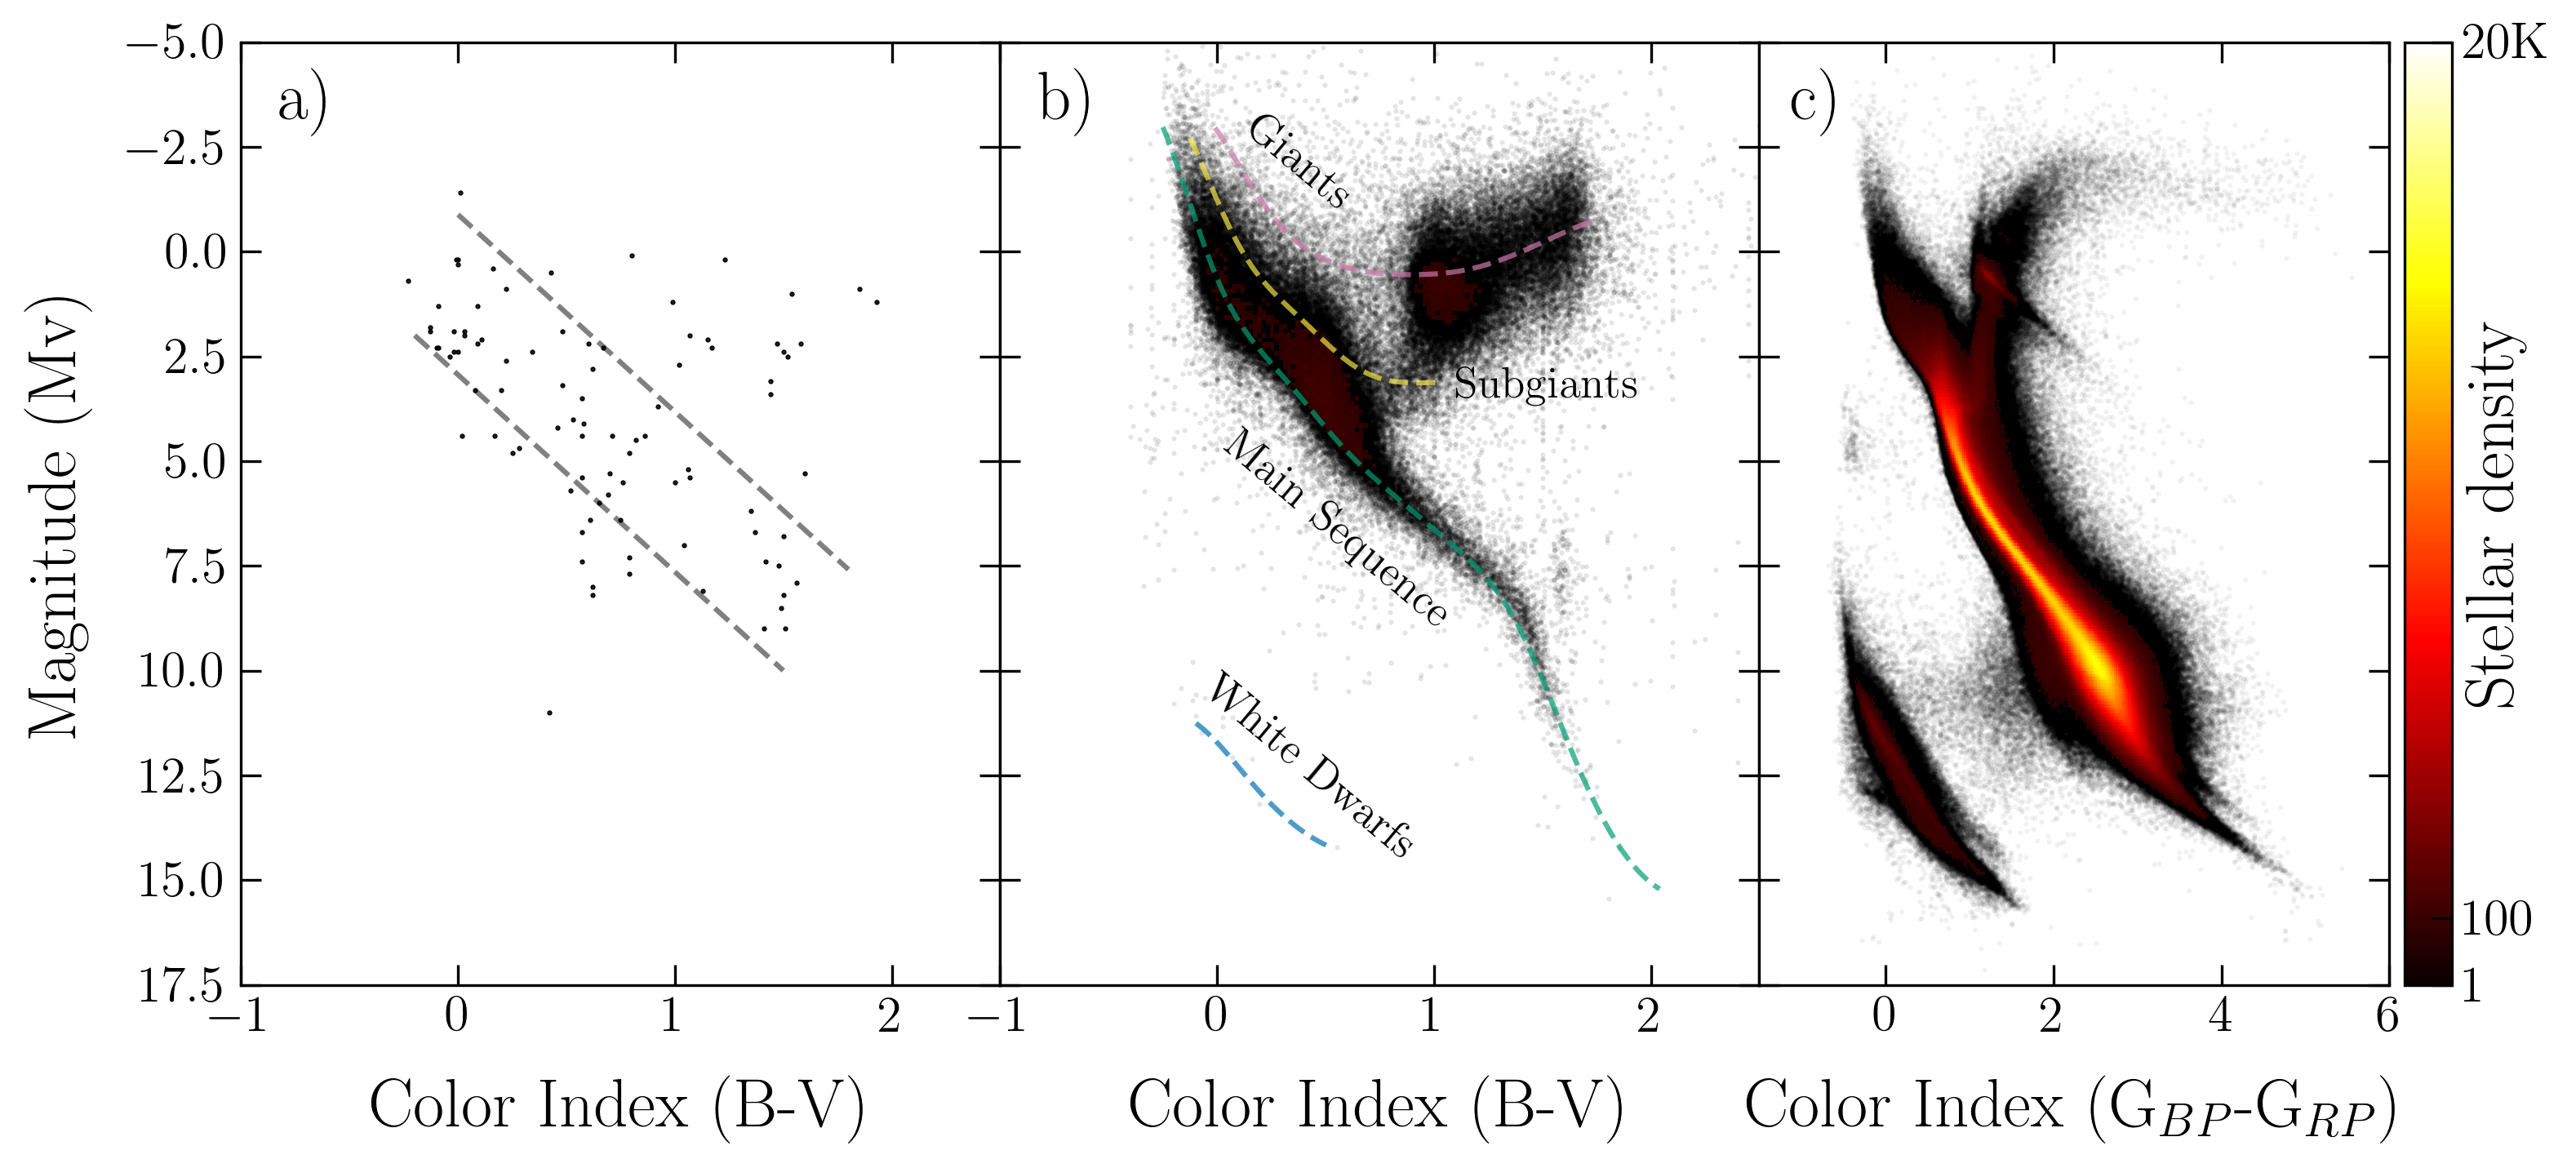
\includegraphics[width=1.2\linewidth]{figures/hr_diagram.png}}
  \caption{\textbf{Observational HR-Diagrams through the ages}: Catalog stars' color index plotted on the horizontal axis and absolute magnitude on the vertical axis. Different regions of the diagram depend on the stars' masses, chemical composition, ages, and stages in the stellar life cycle. The color scale represents the number of stars in each portion of the diagram (black represents lower numbers of stars, and brighter colors correspond to increasingly higher numbers of stars). Panel (a) uses stars cataloged in 1914, panel (b) uses 1993 Hipparcos stars, and panel (c) uses 2022 Gaia stars. 
 \github{https://github.com/avivajpeyi/hr_diagram_past_to_present}}
  \label{fig:HR-diagrams}
\end{center}
\end{figure}

The plot's data points helped Russell demonstrate that the temperature and luminosity of stars are related.
Brighter stars are displayed in the top part of the diagram, while dimmer stars are in the bottom. 
Bluer (hotter-surface) stars are on the left, and redder (cooler-surface) stars are on the right. 
Russell noted that most of the plotted stars fell in a band from the upper left to the lower right.
He indicated this region with lines (the gray dashed lines reconstructed Figure~\ref{fig:HR-diagrams}a).
Russell and Hertzsprung also noticed a separate category of bright but cool red stars in the upper right corner. 
They realized that these bright-cool red stars have a large surface area to produce high luminosity at low temperatures. 
Hertzsprung hence dubbed these as the ``giant" stars.  
Consequently, he named the less-luminous low-temperature red stars "dwarf" stars. 
Russell recognized that the red dwarfs were just the bottom end of the band of stars within the gray lines in Figure~\ref{fig:HR-diagrams}a. 
Hence, Russell extended the grouping of ``dwarf" stars to the entire sequence, the sequence now known as the ``main sequence."
Even though the plot only contained a few stars, it provided Russell with a convenient way to illustrate his ideas about stellar evolution:
\myblockquote{The giant stars then represent successive stages in the heating up of a body and must be
more primitive the redder they are; the dwarf stars represent consecutive stages in later
cooling, and the reddest of these are the farthest advanced.}{Henry Russell, 1914}

  % https://arxiv.org/pdf/1302.0862.pdf
Other astronomers like Eddington also used similar data and the HR diagram to drive some of their theories. 
For example, a decade later, Eddington's mass-luminosity relation would add evidence for stellar evolution down the main sequence.
Soon, the HR diagram became a cornerstone diagram for modern astrophysics, and the concepts of stellar categories led to various advancements in our understanding of stellar physics~\citeme. 
Fortunately, since 1914, technological advances have created much larger samples of stars with well-measured properties, further improving our understanding of stellar physics.


The European Space Agency launched Hipparcos Satellite in 1989\footnote{Hipparcos, an acronym for HIgh Precision PARallax COllecting Satellite, is also reference to Hipparchus, the ancient Greek astronomer who drew up the first accurate star map.}. 
One of the Hipparcos mission's primary goals was to provide a higher resolution observational HR diagram to obtain a detailed structure of stars with $M_v>0$ magnitude. 
In its four years of operation, this satellite cataloged nearly 120,000 stars. 
The Hipparcos catalog stars with low parallax errors, plotted in Figure~\ref{fig:HR-diagrams}b,  show many more details than those in the 1914 HR diagram. 
Firstly, the vertical arm leading off the main sequence and turning to the right is much better defined -- this is the red giant branch indicating that as massive stars get older, they swell and become brighter and redder.
Similarly, the lower left of the diagram shows the white dwarf branch. 
The white dwarf region displays where the less massive stars (like our sun) that cannot undergo a supernova as they get older end up. 
Additionally, if we plotted stars with higher parallax errors, various other categories, such as the bright and super giants, are also visible.

A few years later, Hipparcos's successor Gaia made a considerable leap by cataloging 1.8 billion stars at an accuracy 200 times better than that of Hipparcos. 
Figure~\ref{fig:HR-diagrams}c displays the Gaia stars with low parallax errors obtained in Gaia's third data release. 
This new HR diagram contains over 100 times more stars than Hippacros and allows astronomers to identify more refined details. 
For example, compare the hand full of white dwarfs in the Hipparcos diagram versus the thousands in the Gaia HR diagram.
This increase in white dwarf data has allowed astronomers to study the differences between white dwarfs made with helium cores and hydrogen cores ~\citeme. 
Another exciting detail displayed in the Gaia HR diagram is the imprint of stellar binaries.
These binaries are present both in the main sequence and the white dwarf regions of the diagram (see the second tails at slightly higher magnitudes in both the main sequence and white dwarf regions of the plot).
The Gaia HR diagram appears to have a smaller red giant branch compared to Hipparcos's HR diagram. However, the Gaia HR diagram has many more resolved features, such as the primary and secondary red clumps and the asymptotic giant branch bump. 
The sheer volume of the data made such discoveries possible! 

In addition to data on stellar temperatures and brightness, our catalogs now also contain stellar spectra and time-series data on stellar positions and proper motions.
This data has enabled astronomers to drive theoretical work and make inferences about the nature of stars.
In the following two sections of this chapter, we discuss two more fields where astronomical data has unveiled profound discoveries. 



\section{The dawn of Gravitational wave astronomy}

%% What is a GW 
When some stars reach the end of their lives, they can turn into compact objects such as neutron stars and black holes. 
Some compact objects give away their positions via electromagnetic (EM) radiation due to accretion. 
Others reveal themselves via gravitational wave (GW) radiation emitted due to an oscillating mass quadrupole moment.
Any system with a gravitational quadrupole changing with time produces changes in its gravitational field, resulting in energy emission as gravitational waves.
Gravitational-wave astronomy gives us a new tool to examine the cosmos that complements classic electromagnetic astronomy.
Using gravitational waves, astronomers can research binary black holes and neutron stars that would otherwise be inaccessible.
However, it was only recently that astronomers were able to detect GWs. 

%% History of GW
In 1974, Russell Hulse and Joseph Taylor discovered a pulsar signal using the Arecibo radio telescope.
Measurements revealed that the pulsars' orbital period repeatedly fluctuates every few hours, indicating it is in orbit with a hidden companion.
Hulse and Taylor noted that the orbital period was decaying -- the pulsar and its companion were inspiralling.
After observing the system for another 30 years, they determined that the decrease of the orbital period resulted from the binary releasing gravitational waves, the first observation of gravitational waves.

This indirect detection of gravitational waves paved the groundwork for the Laser Interferometer Gravitational-Wave Observatory, LIGO. 
LIGO was constructed in 1999, but it was not until 2014 that the first gravitational wave from a binary black hole merger was identified.
Since then, the LIGO-VIRGO-KAGRA (LVK) collaboration has recorded several petabytes of data, and astronomers have discovered more than ninety gravitational wave (GW) signals from compact binary mergers.
Individually, these events have provided astronomers with interesting information about various astrophysical objects. 
Taken together, the events form a population that can be studied as a whole. 

\begin{figure}
\begin{center}
  \centerline{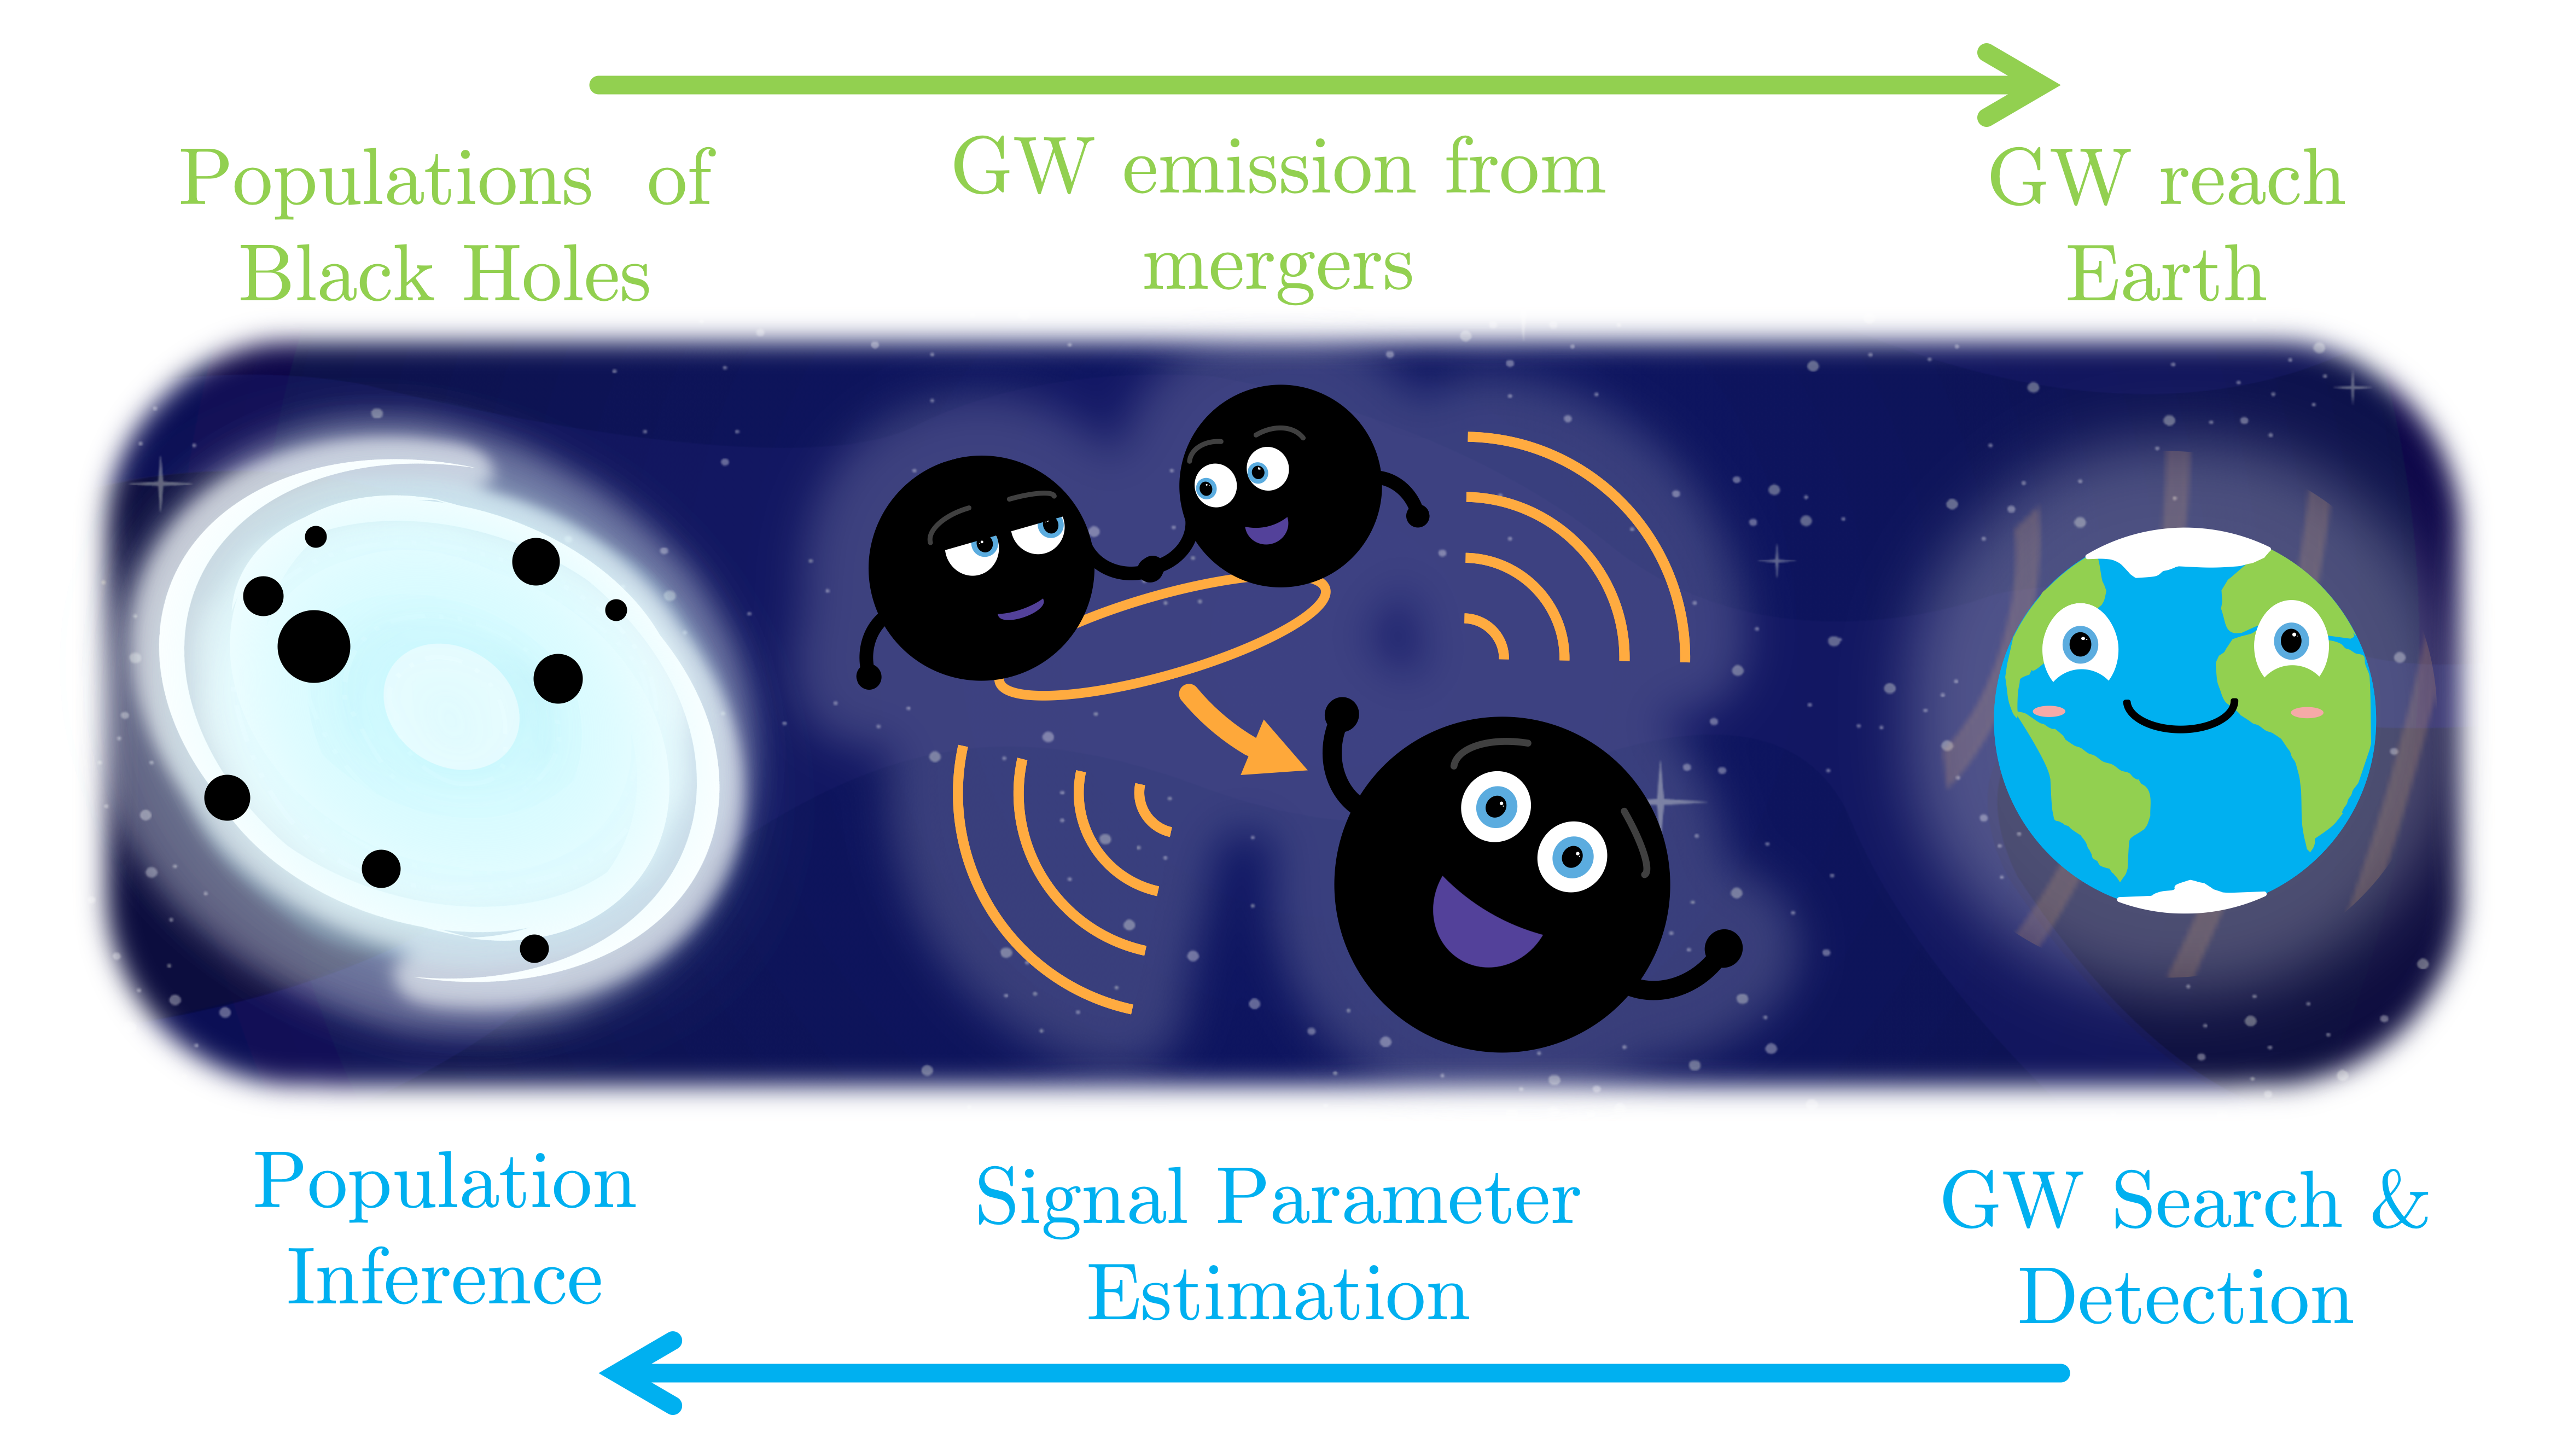
\includegraphics[width=1.1\linewidth]{src/figures/gw_pipeline.png}}
  \caption{\textbf{GW pipeline:} \todo{Remove faces from this schematic} }
  \label{fig:gw_pipeline}
\end{center}
\end{figure}

The following sections introduce the LVK collaborations efforts to (i) search for GW signals from compact binary mergers, (ii) decode the GW signal parameters that describe the merger, and (iii) study the ``demographics'' of the merging black hole populations (each category and its goals are outlined in the schematic Figure~\ref{fig:gw_pipeline}).


\subsection{GW searches}  \label{sec:searches}

As LIGO records data, the data is immediately searched for generic, unmodelled GW transients and modeled GW signals using low-latency search pipelines. 
These searches can identify candidate GW events in near real-time timescales, enabling the possibility of performing follow-up electromagnetic spectrum observations~\cite{abbott2018prospects}.

The unmodeled gravitational wave searches, like the Coherent Wave-Burst (cWB) and BayesWave pipelines, are performed without prior information about expected signal waveforms and instead involve cross-correlating the LIGO and Virgo detector data. 
The cross-correlation is performed on the detector strain time series to look for excess power or bursts in the overlap region between the LIGO Hanford and LIGO Livingston detectors and between the LIGO Hanford and Virgo detectors, respectively \cite{LSC:2016}. 
Such methods are effective at identifying GW transients that can last for
$10^{-3}-10^{1}$s~\cite{abbott2016observing}. 
Unmodeled gravitational wave searches are powerful tools as they may help detect short-duration signals produced by unknown and known phenomena for which we have not yet developed good theoretical models~\cite{Abbott:2016blz}. 
For example, short-duration signals from high mass binary black hole mergers, supernovae, cosmic strings, and unknown astrophysical phenomena as described in~\citep{abbott2018prospects}.

While unmodeled searches look for the unknown,  modeled or targeted gravitational wave searches look for signals from known sources~\cite{abbott2016ligo}. 
Modeled searches for GW signals from the coalescence of compact binary coalescence (CBCs), such as `pyCBC'~\cite{biwer2019pycbc} and
`GstLAL' pipelines~\cite{sachdev2019gstlal},  use prior information about our expectations of GWs in searches. These searches compute the inner product between a gravitational waveform and the data stream and attempt to optimize the inner product by testing different waveforms. 
The different waveforms are chosen from a ``template-bank'' of potential waveforms, where each waveform corresponds to different signal parameters. 


\begin{figure}
\begin{center}
  \centerline{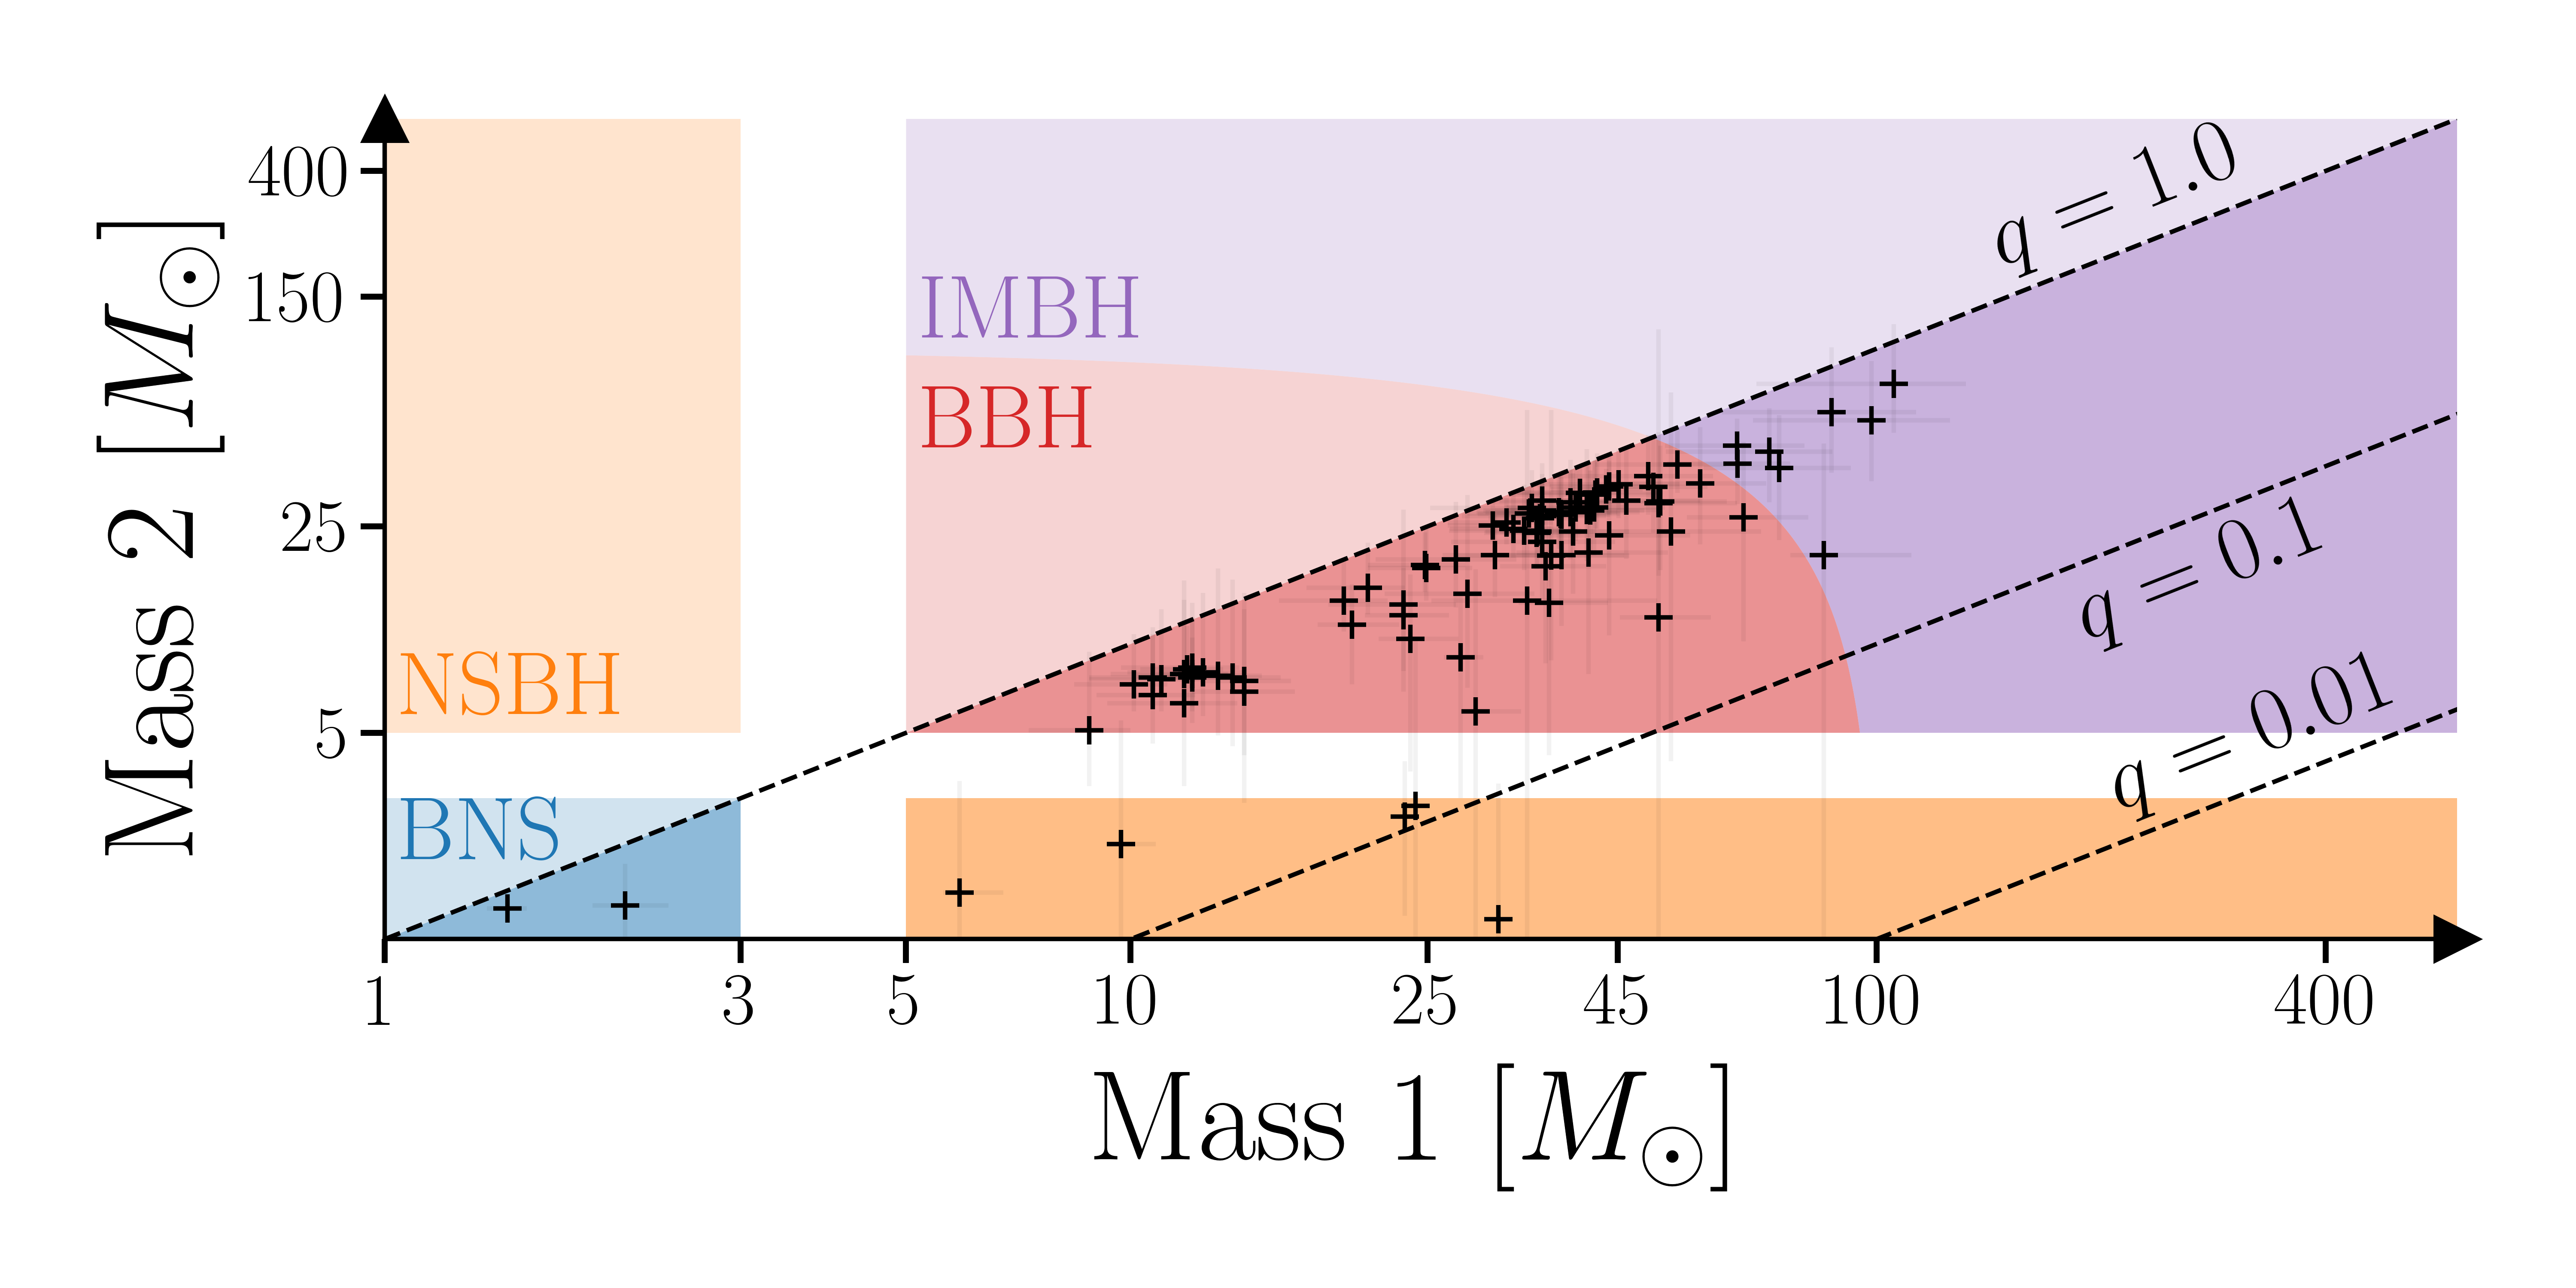
\includegraphics[width=1.1\linewidth]{src/figures/gw_catalog.png}}
  \caption{\textbf{CBC GW merger events:}  \github{https://github.com/avivajpeyi/cbc_gw_catalog_plotter}}
  \label{fig:cbc_mergers}
\end{center}
\end{figure}


These search methods have been able to successfully identify more than 90 CBC GWs, whose masses are plotted in Figre~\ref{fig:cbc_mergers}.
If the detector data contained only gaussian noise and the occasional gravitational wave signal, these search pipelines would successfully identify all signals above some signal-to-noise ratio. 
Unfortunately, some instrumental noise artifacts (glitches) can also be found in the detector data. 
The search pipelines can mistake `glitches' as gravitational wave signals. 
Hence, the search pipelines also test signal coherence and compute `ranking statistics' to determine the statistical significance of candidates to prevent false positives. 

Efficient signal detection requires a ranking statistic that extracts the most information from the data to discriminate between noise and weak astrophysical signals.  
However, existing CBC searches are not optimal: they do not incorporate knowledge of all features that may distinguish GWs from noise. 
Moving toward an optimal statistic is a great challenge, but one toward a better ranking statistic may be to demand that foreground triggers in two or more detectors should be better described
as coherent gravitational-wave signals rather than incoherent glitches.
Importantly, it is not enough to provide some measure of coherence: one must also prove that an incoherent model is not more successful at
describing the data. 

The Bayesian coherence ratio, `BCR', proposed by \citet{bcr_paper} can help take a step towards this optimal statistic. 
As short-duration gravitational wave signals such as those from intermediate-mass black holes are the most challenging to distinguish from glitches, in Chaper~\ref{cp:imbh}, we investigate the usefulness of the `BCR' as a ranking statistic. 

\subsection{GW Signal Parameter Estimation}

The core of parameter estimation in gravitational waves is Bayes' theorem. 
Given a model with parameters $\theta$, some data $d$ and the \textit{likelihood} $\mathcal{L}(d|\theta)$ of the data given the model, Bayes' theorem states that the \textit{posterior probability} $p(\theta|d)$ of model parameters given the data is 
\begin{equation}
{p(\theta|d)} = \frac{\mathcal{L}(d|\theta)\pi(\theta)}{\mathcal{Z}}\ , \label{eq:bayeTheorem}
\end{equation}
where $\pi(\theta)$ is the \textit{prior} probability of the model parameters, and $\mathcal{Z}$ is the marginalized likelihood known as the
\textit{evidence}. 
The evidence is a single number that describes how well a model fits the data and is given by 
\begin{equation}
Z(d) = \int_\theta \mathcal{L}(d|\theta)\pi(\theta)d\theta\ .
\label{eq:evid}
\end{equation}
As the evidence is a probability of the data irrespective of model parameters, it is a valuable quantity to compare various models and determine which model better describes some data.

Using gravitational wave models and equation~\ref{eq:bayes}, astronomers can compute the posterior probability of gravitational wave model parameters given some data containing a gravitational wave signal~\cite{abbott2018prospects}.
However, as CBC GW models can use more than 11 parameters to describe a signal, evaluating the posterior probability for gravitational waves is computationally expensive. 
For example, consider evaluating the posterior probability at $10$ gridpoints for each of the $11$ GW parameters.
This case results in a huge number of $10^11$ points to evaluate the posterior.
Furthermore, one would need to use many more grid points to represent the continuous parameter space accurately.
Finally, gravitational wave models incorporate complex physics, so they can be computationally slow to evaluate. 
Altogether, evaluating the posterior overall points of parameter space is an insurmountable computational challenge.

An alternative way to estimate the posterior over a large parameter space is to utilize approaches such as Markov chain Monte Carlo (MCMC) and Nested Sampling to produce multivariate draws from the posterior. 
These methods can also be parallelized to speed up the inference process. 
For a detailed discussion on the parallelization of nested sampling and how it can boost gravitational wave inference, refer to Chapter~\ref{cp:pbilby}. 


\subsection{Interpretting GW signals}

After GW searches and parameter estimation pipelines  identify and characterize signals, astronomers can begin interpreting the inferred parameters.
Mass and spin inferences help determine where (eg, isolated-space, globular clusters, or active galaxies) these binaries form and merge.
Each observation's inferred parameter can reveal the binary's formation pathway.

For example, consider the inferred parameters for GW190521 and GW190425. 
GW190521's parameters show that the signal originated from an asymmetric BBH merger with masses of $85^{+21}_{-14}M_{\odot}$ and $66^{+17}_{-18}M_{\odot}$ \citep{Abbott:2020tfl}.
The remnant object was the first direct detection of an IMBH with a mass surpassing the pulsational-pair instability mass gap.
Due to its large initial masses, some believe this may be a second-generation merger and hence is improbable to be a field merger. 
On the other hand,  parameter estimation of GW190425 suggests the event's binary had a non-circular orbit, indicating it may have come from a globular cluster.

In a similar vein, the community has recently been discussing GW151226. 
Initial research concluded that GW151226 resulted from a CBC with conventional masses and spins, as seen in Figure~\ref{fig:gw151226_cases} (case A).
However, recent work suggests that the GW emerged from a peculiar system: asymmetric BBH merger with even spins misaligned (case B).

%% GW151226 Figure
\begin{figure}
\begin{center}
  \centerline{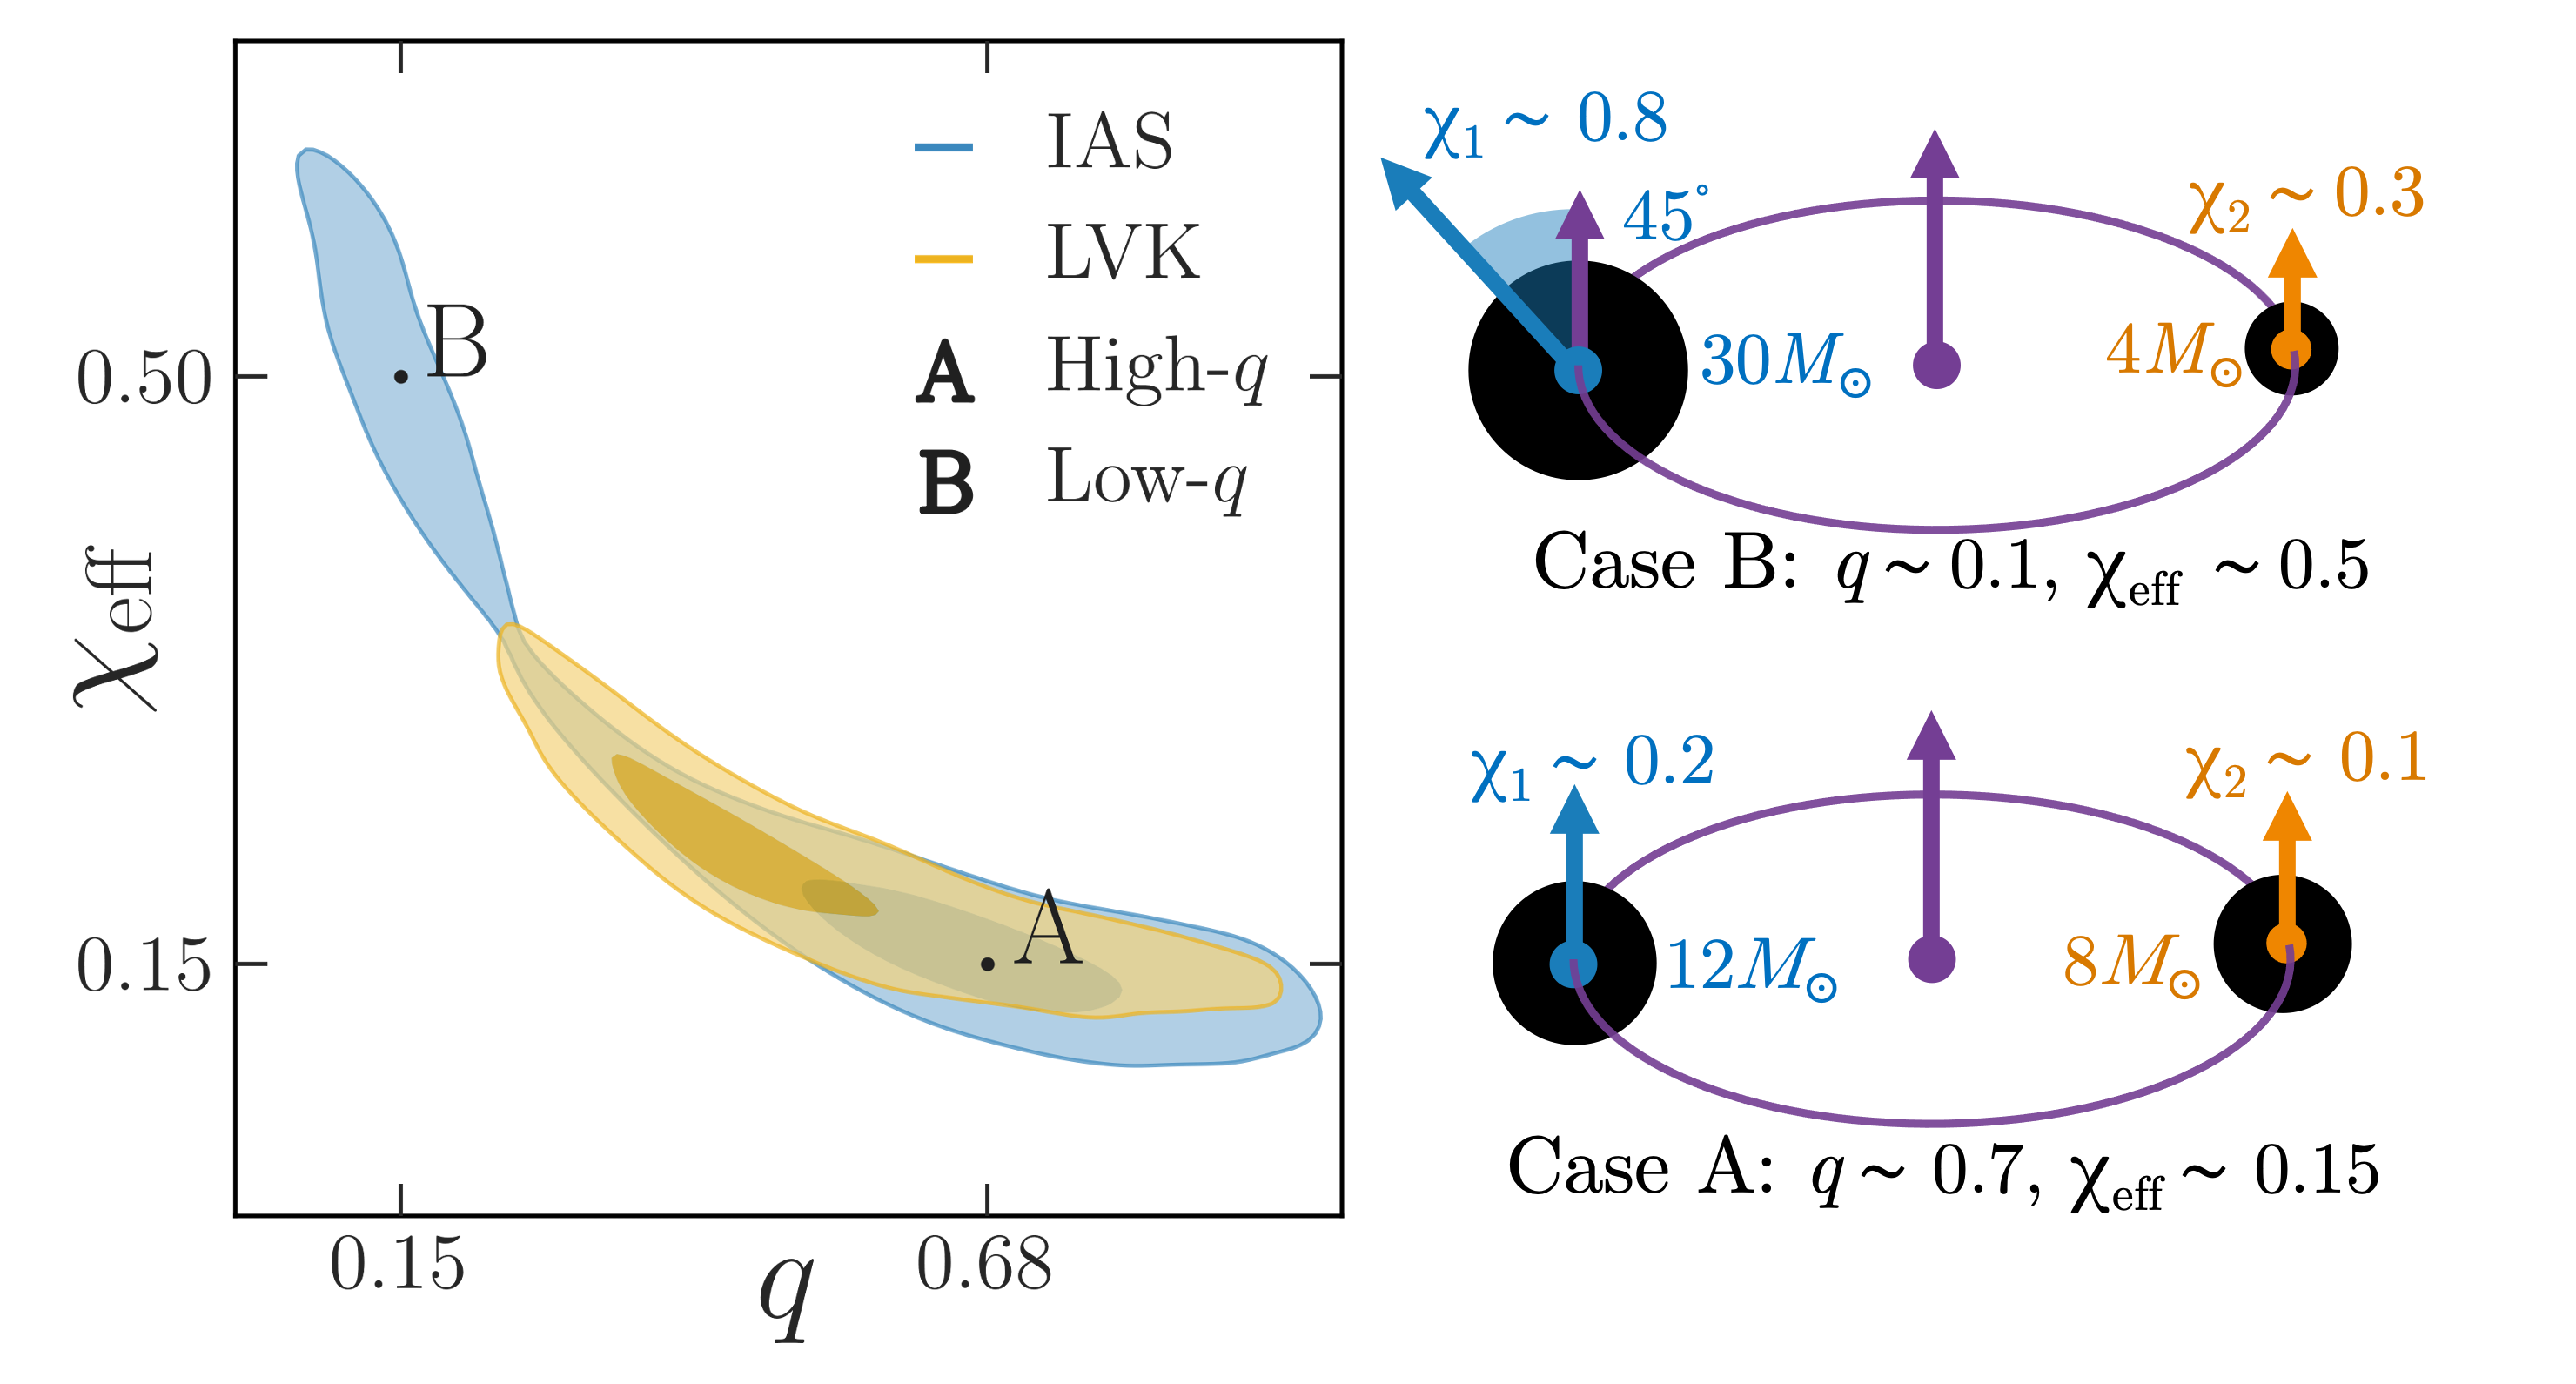
\includegraphics[width=1.1\linewidth]{src/figures/gw151226_cases.png}}
  \caption{\textbf{GW151226 Cases:}  }
  \label{fig:gw151226_cases}
\end{center}
\end{figure}

It's uncertain which of these cases is most likely, making it difficult to establish this event's formation channel.
Chapter~\ref{cp:deep_followup} presents a ``deep follow-up'' tool to determine which case is  more probable.
It employs Bayesian model selection to evaluate the posterior odds of two points by computing the points' marginal likelihood.
The posterior odds for case A versus B are near 1, reflecting that it is valid to interpret GW151226's binary to have been from either case.

\subsection{GW population inference}

With many GW events, astronomers can also study the ensemble properties of merging systems, such as how masses and spins of all detected BHs are distributed, using hierarchical inference techniques.
The LVK has used several hypotheses in hierarchical inference studies to map ensemble mass and spin distribution features to astrophysical processes  described by stellar evolution and population synthesis models.
For example, recent work on the black hole spin population has examined computing the fraction of signals expected to result from isolated-field binary mergers versus dynamical binary mergers.
In Chapter~\ref{ch.agn}, we look into another binary merger channel: the active galactic nuclei (AGN) channel.
AGNs are promising environments for the assembly of merging binary black hole systems with large masses (e.g. GW190521~\cite{gw190521_agn}), asymmetric masses (e.g. GW190521~\cite{gw190425_agn}), and a variety of spin configurations~\cite{agn_spin_population_models}. 

\begin{figure}
\begin{center}
  \centerline{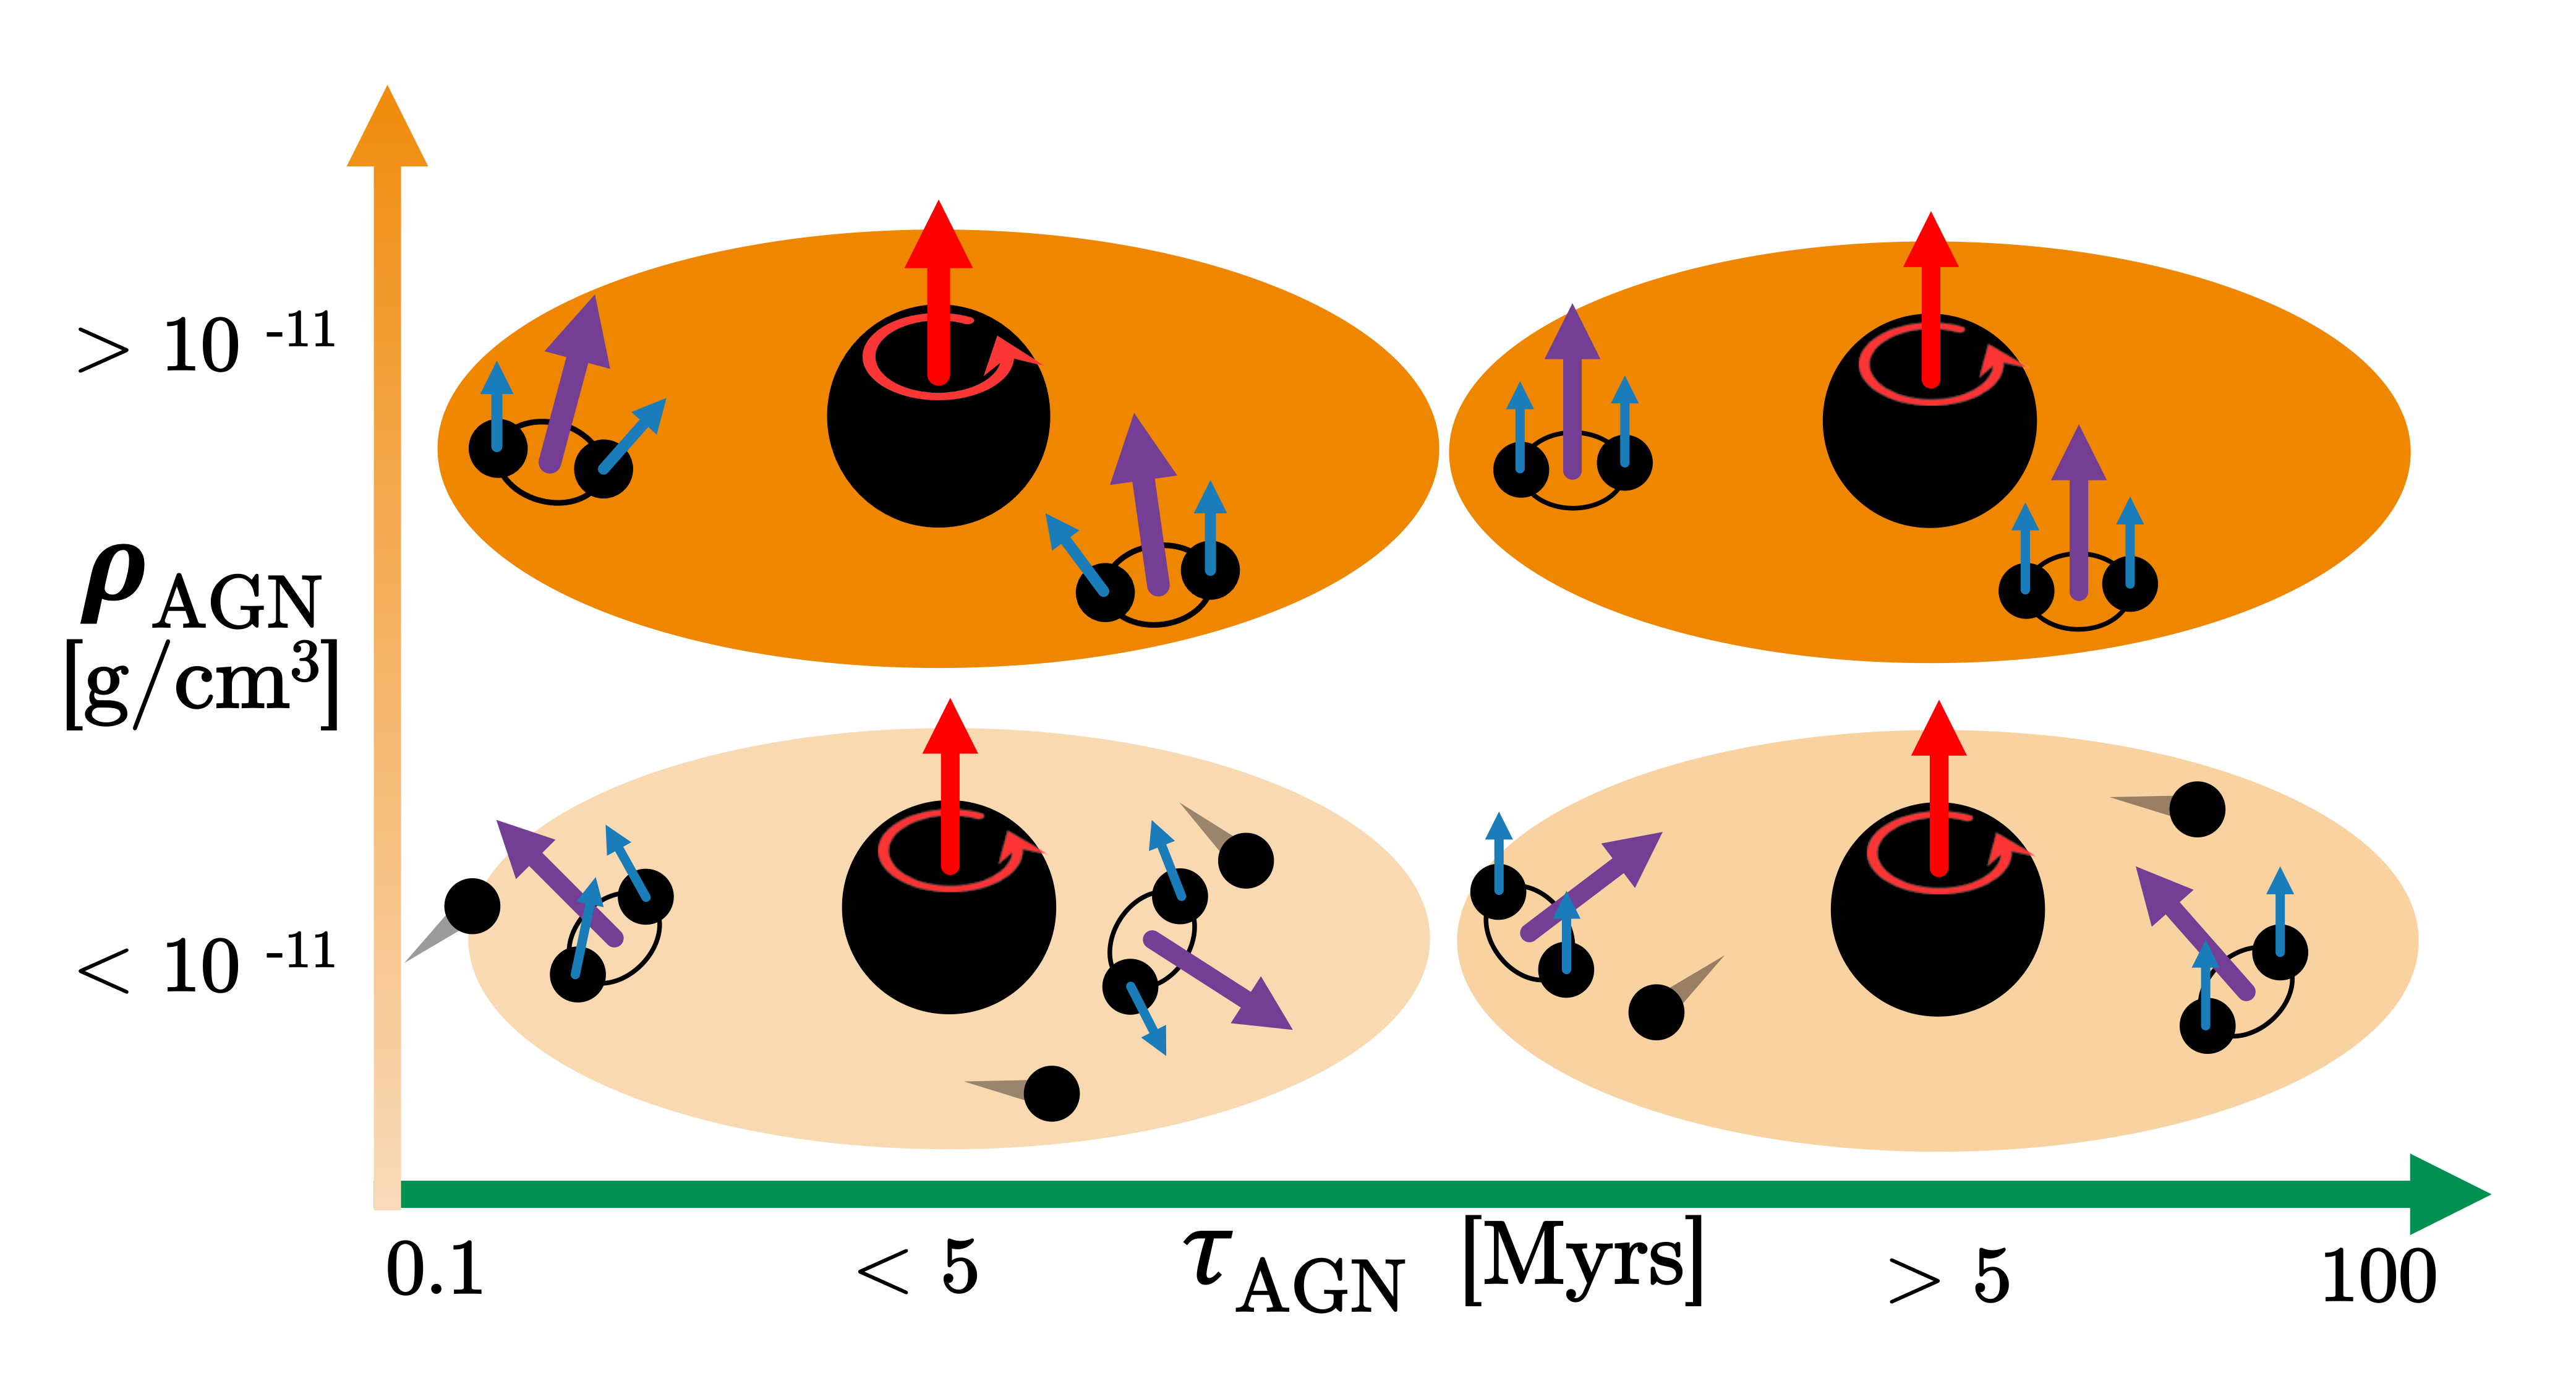
\includegraphics[width=1.\linewidth]{src/figures/agn_spins.png}}
  \caption{\textbf{AGN BBH-spins:} Different AGN age $\tau_{\rm AGN}$ and density $\rho_{\rm AGN}$ values can lead to different binary black hole spins. }
  \label{fig:agn_spins}
\end{center}
\end{figure}


In Chapter~\ref{ch.agn} we draw on simulations of BBH systems in AGN to propose a phenomenological model for the distribution of black hole spins of merging binaries in AGN disks. 
The model incorporates distinct features that make the AGN channel potentially distinguishable from other channels, such as assembly in the field and globular clusters. 
The model parameters can be mapped to the age $\tau_{\rm AGN}$ and density $\rho_{\rm AGN}$ of AGN disks. 
A schematic illustration of the model is presented in Figure~\ref{fig:agn_spins}. 
In the Figure's top right corner, where the AGN is old and dense, the BBH orbital angular momentum and component BH spins align with the central SMBH spin. 
Conversely, all spins are misaligned in the lower left, where the AGN is young and dilute. The other two corners represent unique spin orientations described in further detail in Chapter~\ref{ch.agn}.
We estimate how these different populations of binaries in AGNs can be distinguished.
If most merging black holes are assembled in AGNs, future gravitational-wave observations may provide insights into the dynamics of AGN disks.

\section{The hunt for exoplanets}

Humans have long sought for exoplanets, planets beyond our solar system, to answer questions like: how did the planets in our solar system form? Are Earth-like planets common? And, the biggest yet -- is there life beyond Earth? 
The answer to the last question will change humankind forever, whether it reveals a universe replete with rare and fragile life, or no life.
Nevertheless, just as our ability to locate faraway stars or detect gravitational waves was constrained by technology until relatively recently, so was our ability to investigate exoplanets.
Now, thanks to the Kepler and TESS satellites, astronomers have found thousands of exoplanets.
Although no traces of life have been identified, scientists have learned that these worlds vary greatly in size and temperature and are composed of the same elements as the planets in our solar system.
This section reviews the hunt for exoplanets, and some of what we have learned from the exoplanets found so far.

\section{Planets beyond the solar system: search and discovery}

Sometimes, serendipity plays a role in science.
The first  exoplanet observation is one such incident.
As the world trembled from the onset of World War I in 1917, Walter Adams was recording the spectrum of a white dwarf star on a glass plate.
The spectrum of this star contains unusually heavy components, such as magnesium and iron.
These contaminants could not have evolved naturally within the star, thus they must have originated from the shattered remains of an exoplanet.
Unfortunately, Adams was unaware of this, and his finding stayed in the archives until 2016, when Jay Farihi discovered and correctly interpreted Adam's work.

Since Adams' observations, many scientists have reported discoveries of exoplanet candidates.
Unfortunately, all candidates were disproven, until 1992 when Aleksander Wolszczan and Dale Frail published their work on a bizarre system. 
Wolszczan and Frail were investigating  pulsar PSR B1257+12's periodic timing variations.
After extensive investigation, they concluded the periodicity was due to two planets orbiting the pulsar. 
Astronomers were initially surprised by this planetary system because they anticipated that supernovae that generated pulsars would kill or eject any planets in orbit via a shockwave. 
Therefore, the scientists hypothesised that these two planets may have formed when the destroyed planets' gas and dust accumulated around the pulsar after the supernova.
Although exciting, Wolszczan and Frail's exoplanet was not what scientists were on the hut for -- the search for the first exoplanet orbiting a sun-like star was still on.
Exciting as it was, Wolszczan and Frail's exoplanet was not what scientists were seeking; the hunt for the first exoplanet orbiting a sun-like star continued.
Only 3 years later, the hunt resulted in the discovery of exoplanet ``51Pegasi b'' by Didier Queloz, a doctoral student, in 1995.
Queloz discovered this massive exoplanet with an orbit of 4 days using a technique called the ``radial-velocity'' method, in which the small wobble of a star is measured due to the gravitational pull of an orbiting planet. 


\begin{figure}
\begin{center}
  \centerline{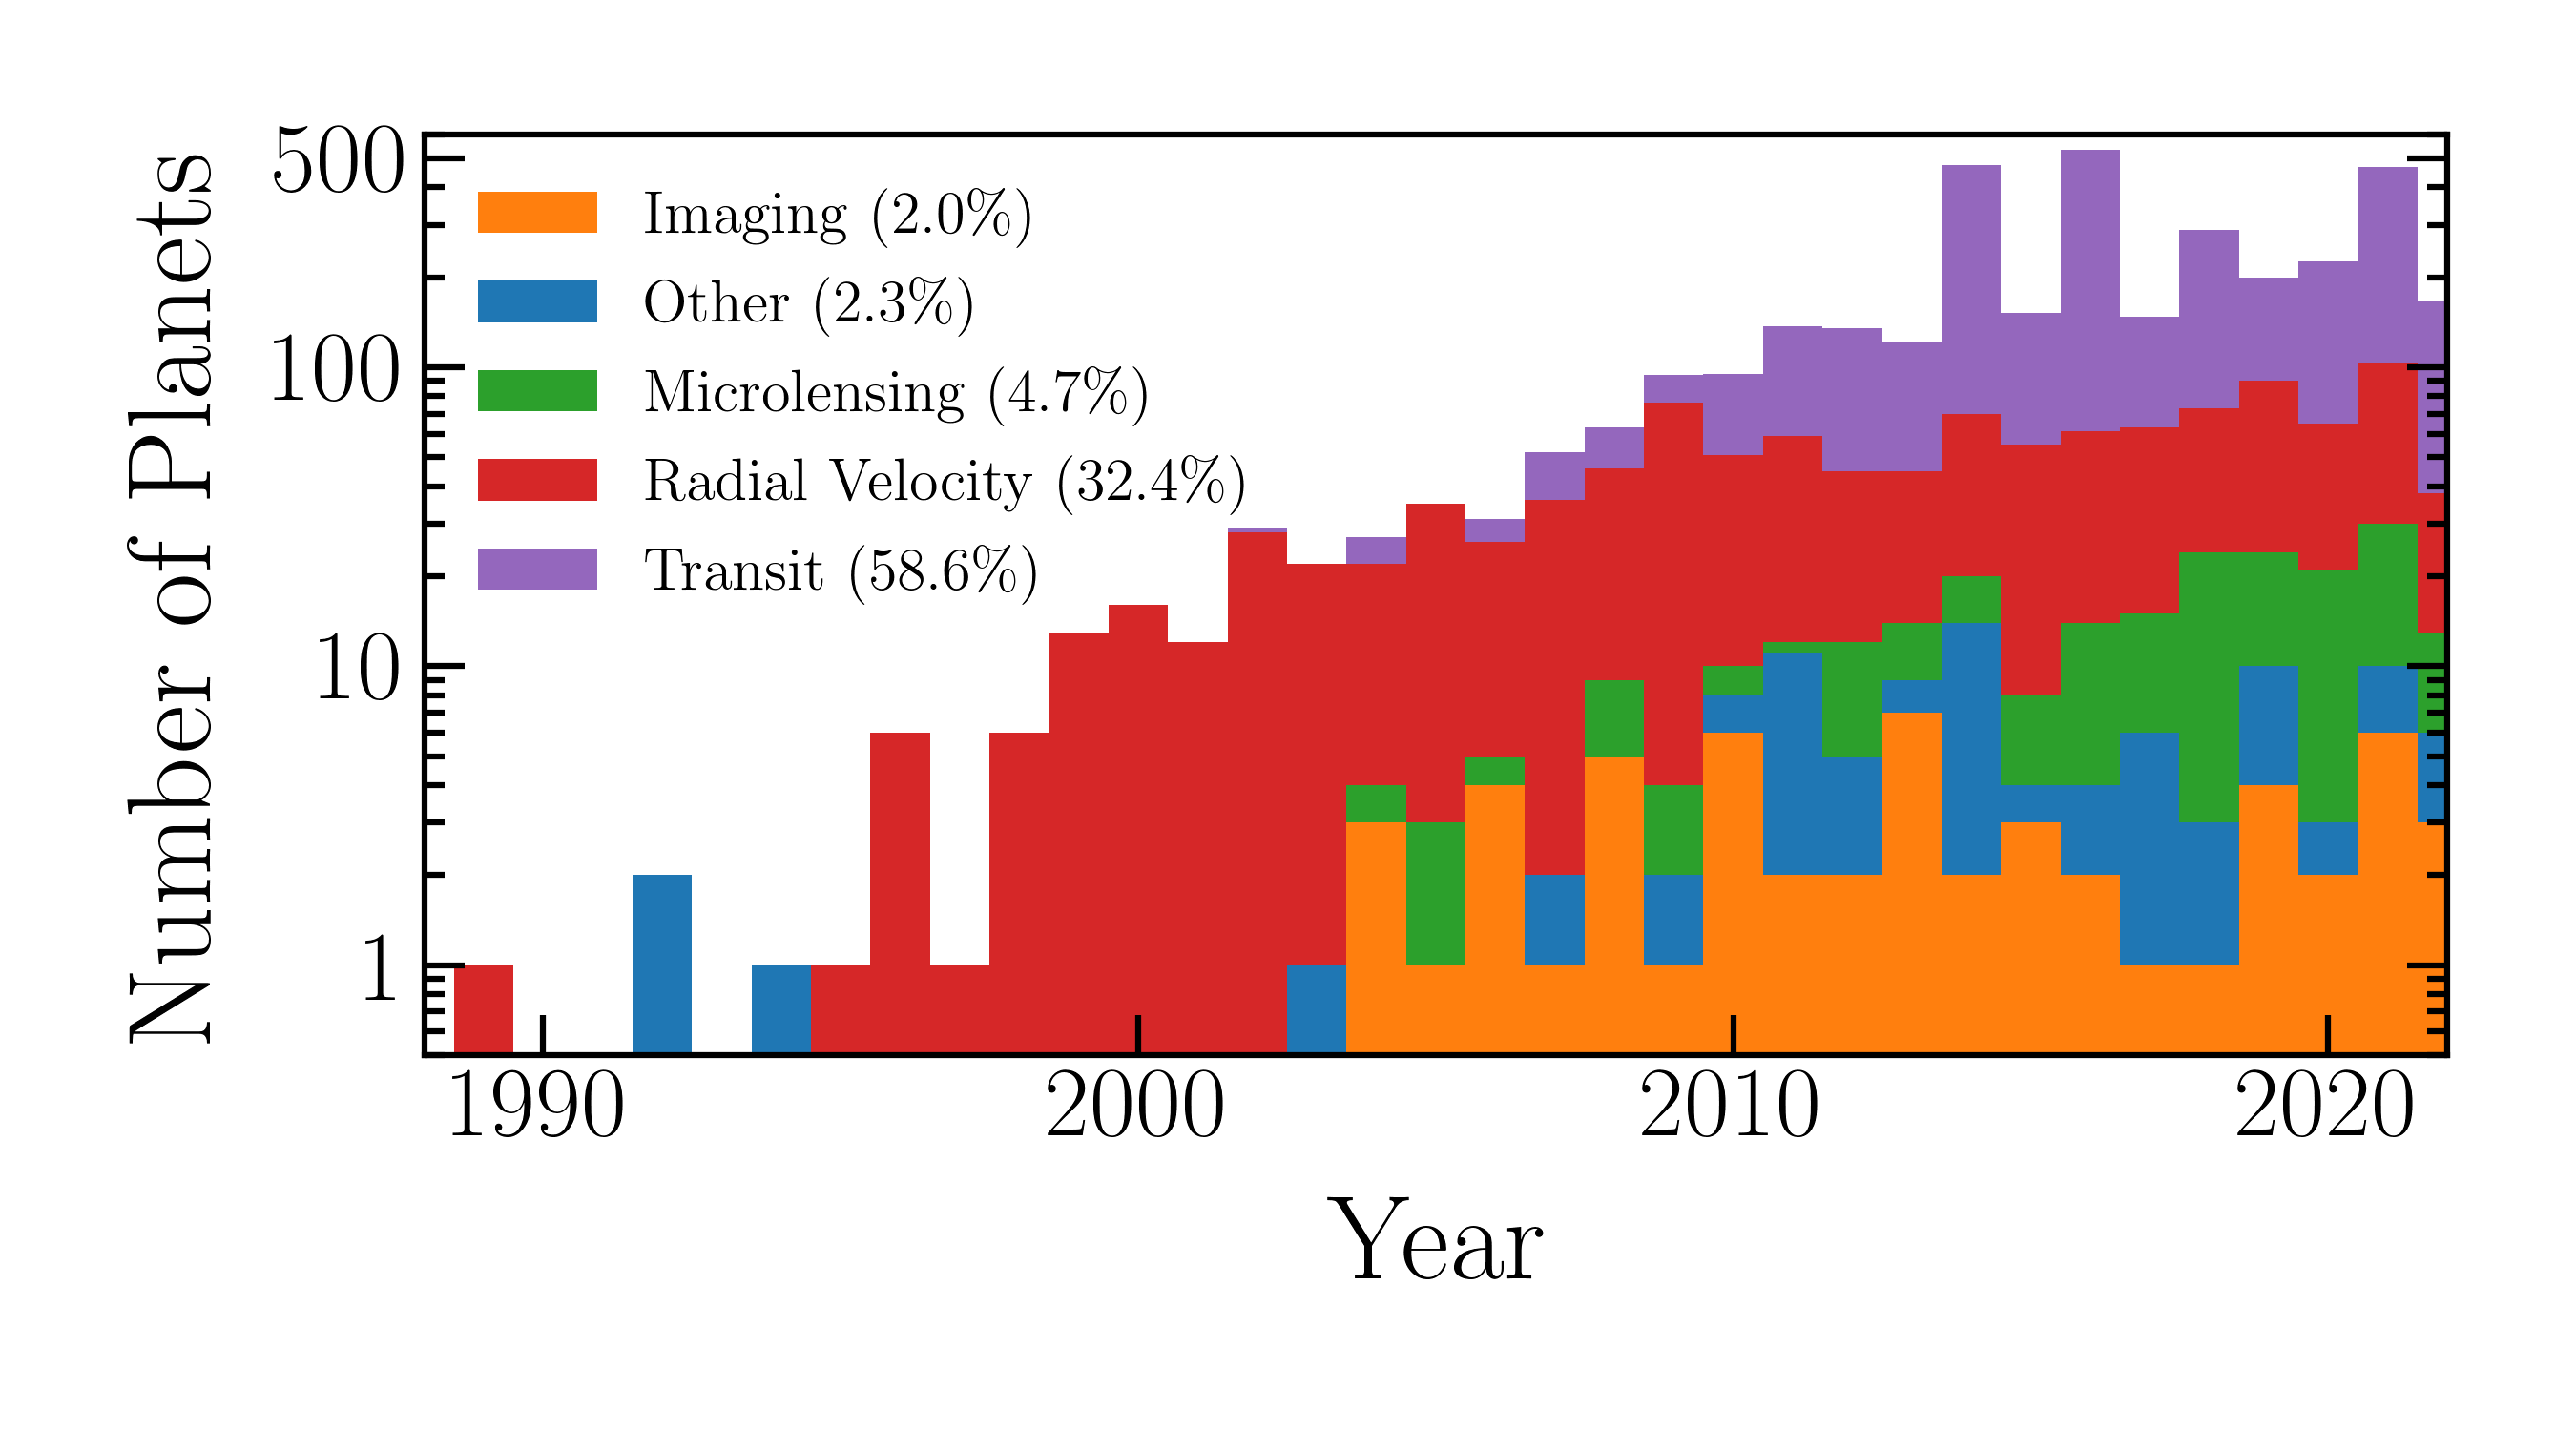
\includegraphics[width=1.\linewidth]{src/figures/confirmed_planets_vs_time.png}}
  \caption{\textbf{Exoplanet detections over time:}  \github{https://github.com/avivajpeyi/exoplanet_catalog_plotter}}
  \label{fig:exo_detections_over_time}
\end{center}
\end{figure}


Several other exoplanets with radial velocity were discovered after 1995.
In 1999, \citet{charbonneau1999detection} utilised a network of three 10-cm telescopes\footnote{Some of these telescopes were set up in parking lots!} to focus on the star of a recently discovered exoplanet.
They identified the exoplanet using the transit method, which looks for periodic dips in a star's brightness caused by an orbiting planet blocking some light~\cite{charbonneau1999detection}.
Soon, the transit method became the most effective technique for discovering exoplanets.

Figure~\ref{fig:exo_detections_over_time} plots the number of exoplanet discoveries from 1989 to 2022. 
The graphic illustrates that the transit approach has discovered the most extrasolar planets, followed by the radial velocity method.
The data also indicate that the number of exoplanet discoveries has increased significantly over time.
Launches of the Kepler and TESS satellites helped to boost the number of detections.

Launched in 2009, Kepler observed 530,000 stars in the Cygnus constellation and confirmed over 2,600 exoplanets. 
Prior to its retirement in 2018, analysis of Kepler's data established that there are more planets than stars in our galaxy~\cite{Swift_2013} with 20-50\% of stars have small (potentially Earth-like) planets~\cite{Fressin:2012:Natur, Petigura:2013:PNAS}, and that there appear to be different categories of planets~\cite{Traub:2012:ApJ, Morris:2017:ApJ, Yu:2017:ApJ}.
Finally, Kepler data showed that the Solar System was the most peculiar planetary system discovered to date~\cite{Weiss:2018:AJ}. 
The following sections delve into some of these discoveries.

\section{From Hot Jupiters to Habitable Super-Earths}


\begin{figure}
\begin{center}
  \centerline{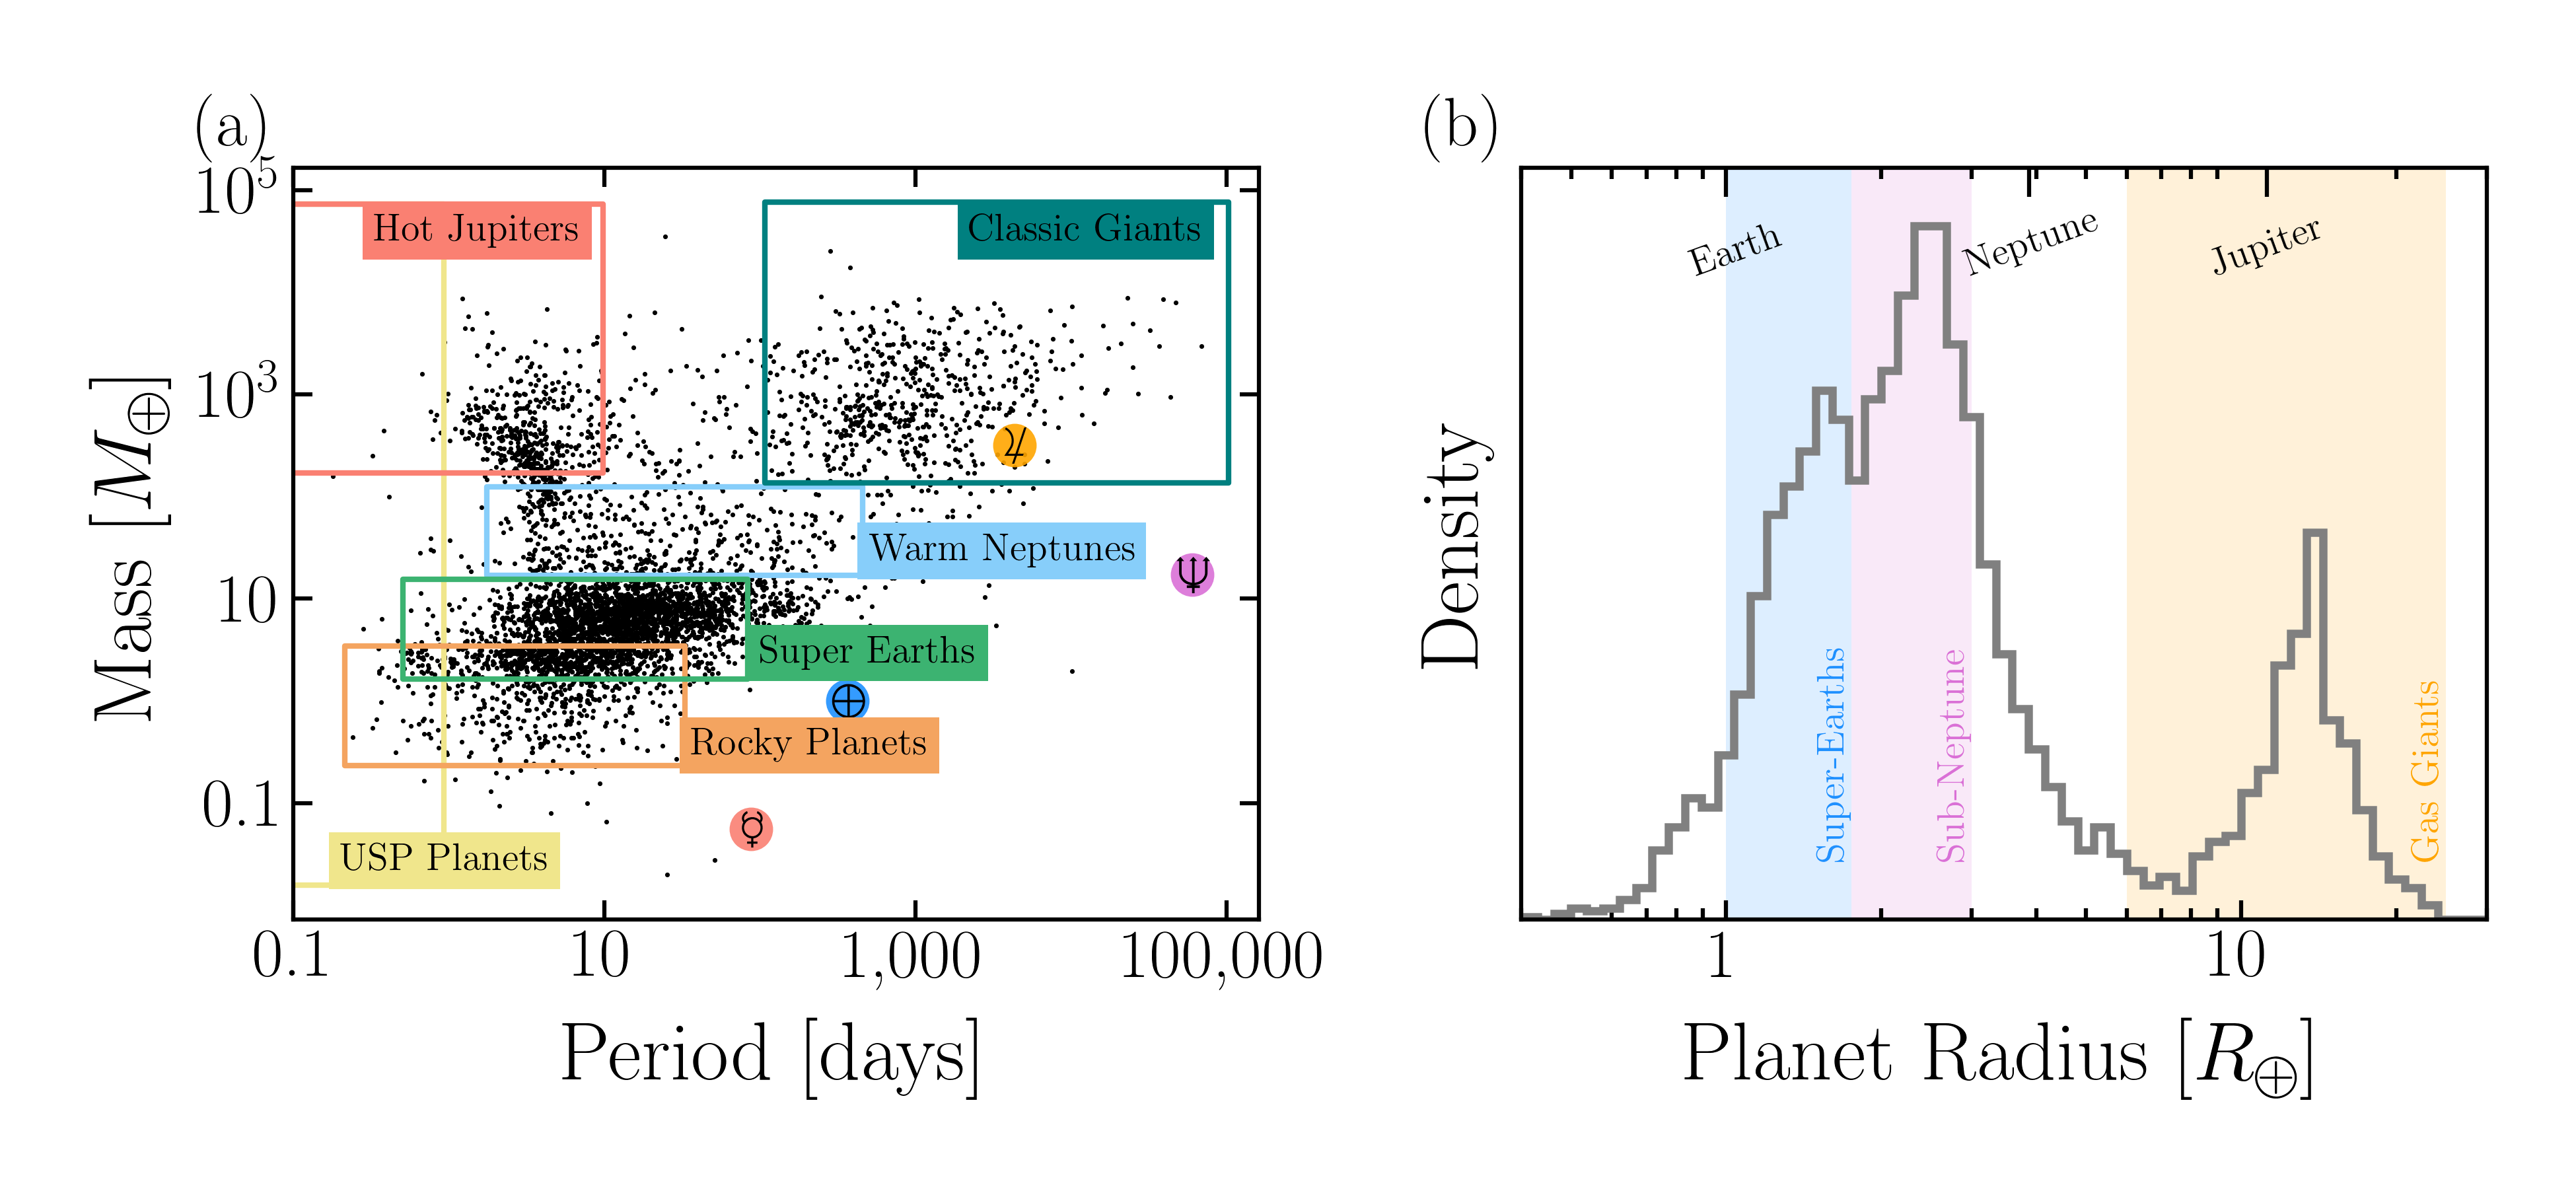
\includegraphics[width=1.1\linewidth]{src/figures/scatter_categories.png}}
  \caption{\textbf{Exoplanet Categories:}  \github{https://github.com/avivajpeyi/exoplanet_catalog_plotter}}
  \label{fig:exo_categories}
\end{center}
\end{figure}

% 

\paragraph{Large versus small planets:}
Before Kepler's launch, most exoplanets identified (using radial velocity) were hot, massive gas giants, top region of Figure~\ref{fig:exo_categories}a~\cite{kepler_mission}.
These large planets were so close to their host stars that they caused a pronounced ``wobble'' in the stellar spectra, making them stand out in radial velocity exoplanet searches~\cite{kepler_mission}.
Therefore, estimating  the proportion of terrestrial (planets with radii $R\sim1-3\ R_{\oplus}$)  and jovian planets  ($R\sim10-20\ R_{\oplus}$) was one of Kepler's primary objectives.

Kepler was successful in this mission as its data revealed many jovian and terrestrial planets, both found via the transit method~\cite{kepler_mission}.
Figure~\ref{fig:exo_categories}b shows that there are a far greater number of small exoplanets (radii less than Neptune's) than the giant exoplanets (radii above Neptune).
The most common planets have radii in the super-Earth and sub-Neptune categories. 
This makes our solar system rather peculiar: the most common types of planets in the Galaxy are completely absent from our solar system and were unknown until Kepler’s survey~\cite{Oppenheimer:2016:Sci}.

The region between the super-Earths and sub-Neptunes in Figure~\ref{fig:exo_categories}b also contains an interesting gap, called the photoevaporation valley (also known as the Fulton gap)~\cite{Owen:2013:ApJ, VanEylen:2018:MNRAS}. 
This valley occurs due to atmospheric stripping of 1.5-2 $M_{\oplus}$ planets, leaving a population of stripped, rocky planets close to their stars (the super-Earths). 
The planets that avoid stripping form a second population of thick-atmosphere planets farther away from their stars (the sub-Neptunes).

It is important to note that even the transit approach with Kepler data has biases — it has trouble finding planets with radii $R<R_{\oplus}$ and lengthy periods~\cite{kepler_mission}.
The dearth of small-sized long-period planets can be seen in the bottom right side Figure~\ref{fig:exo_categories}a.


\begin{figure}
\begin{center}
  \centerline{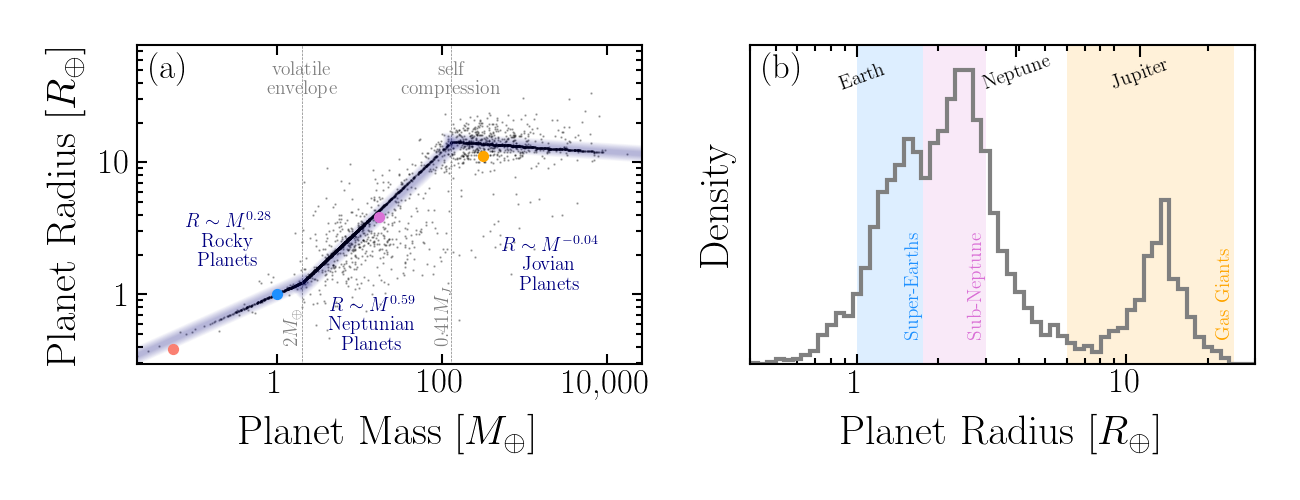
\includegraphics[width=1.1\linewidth]{src/figures/radii_and_mass_relations.png}}
  \caption{\textbf{Digging into exoplanet mass and radius distributions:} 
  Fig on left inspired by \cite{Chen:2017:ApJ}
  Habitable zone fig on right 
  \github{https://github.com/avivajpeyi/exoplanet_catalog_plotter}}
  \label{fig:exo_mass_radius_relations}
\end{center}
\end{figure}



\paragraph{Looking for signs of life:}
In addition to identifying different-sized planets, Kepler's mission was designed to investigate habitable worlds~\cite{kepler_mission}.
Scientists define habitable worlds as solid planets with a wide enough orbit to form liquid water on their surface (the star's habitable zone).
This section discusses these two conditions.

Density estimates can indicate if the planet is solid.
By estimating exoplanet masses (using radial velocity measurements) and radii (using the transit method), scientists can compute the density and infer whether a planet is composed primarily of rock, water, or gas.
The mass and radii of planets are plotted in Figure~\ref{fig:exo_mass_radius_relations}a. 
Planets with masses below $2\ M_{\oplus}$ (or $R < 1.23 R_{\oplus}$) are termed \textit{Terran worlds} due to their rocky, Earth-like composition (e.g., Earth, Mercury, Venus, Mars)~\cite{}.
Next are the \textit{Neptunian worlds}, which have a gaseous ``volatile envelope'' (e.g. Saturn, Uranus, and Neptune)~\cite{Chen:2017:ApJ}.
The final group consists of gas giants, or \textit{Jovian worlds} (e.g. Jupiter).
Figure~\ref{fig:exo_mass_radius_relations}a shows that additional mass increases the radii of terrestrial and Neptunian planets, but decreases the size of gas giants due to ``self-compression" by gravity.
Using planets with mass and radius measurements, scientists constructed a mass-radius power-law relation, represented in Figure Xa by the broken purple power-law~\cite{Chen:2017:ApJ}.
This power-law was utilized to deduce mass/radius predictions for planets with a radius/mass measurement — the dense cluster of planets in the center of the purple power-law~\cite{Chen:2017:ApJ}.
In turn, the mass and radii of numerous exoplanets have suggested a population of rocky planets~\cite{kepler_mission}.
However, the question of if the planets are within the habitable zone is more complex.


Initial theory suggested that a star's habitable zone (HZ) is a function of its mass. 
However, improved models demonstrate the importance of incorporating a myriad of additional parameters like planetary rotation~\cite{Yang:2014:ApJL},  mass~\cite{Kopparapu:2014:ApJL}, albedo, atmospheric heating~\cite{Kasting:2011:AsBio}, and others~\cite{Kopparapu:2013:ApJ, Kopparapu:2014:ApJL, Shields:2014:ApJL}. 
Plotted in Figure~\ref{fig:exo_mass_radius_relations}b is \citet{Kopparapu:2014:ApJL}'s (slightly outdated) habitable zone fit, containing over 250 exoplanets.
Although not all of these planets in the HZ will truly be habitable, these planets act as potential candidates for future follow-up. 
Furthermore, recent work by 
\citet{Bryson:2021:AJ} combining Kepler exoplanet data with Gaia stellar data estimated that our galaxy contains over 3 hundred-million potentially habitable planets.
Hence, there should be a lot more than just 250 habitable exoplanet candidates.


\section{Passing the baton from Kepler to TESS }
As seen in the preceding sections, Kepler's mission was a tremendous success and led to the discovery of thousands of exoplanets.
However, the Kepler mission was not devoid of difficulties.
The mission ran into issues when two of the four reaction wheels failed (required for precise alignment). 
This malfunction concluded Kepler's primary mission 2013.
Kepler continued to operate until its fuel ran out in 2018.

A few months after, TESS, the Transiting Exoplanet Survey Satellite, replaced Kepler as the primary spacecraft to discover new exoplanets.
While Kepler surveyed less than 1\% of the sky, TESS has surveyed over 75\% of the sky and will get full coverage over the next few years. 
Additionally, TESS observes brighter stars than Kepler to enable follow-up on some exoplanets via ground-based telescopes.  
So far, TESS has found over 250 confirmed planets and has over 5,887 candidate exoplanets. 
To aid in the promotion of some of these candidates to confirmed planets, we analyse all the candidates with a Bayesian inference framework. 
This work is presented in Chapter~\ref{cp.tess}.


\section{Overview}
The remainder of the dissertation is structured as follows.
Chapter~\ref{ch.bcr} presents a Bayesian-inspired ranking statistic to aid in the search for gravitational waves from intermediate-mass black holes.
A review on other methods to detect IMBHs is presented in Appendix~\ref{apdx.imbh}.
Chapter~\ref{ch.pbilby} introduces a parallelized nested sampling library for gravitational wave parameter estimation.
This covers the parameter estimation method used in subsequent gravitational wave chapters. 
Chapter~\ref{ch.deep} documents a new method of settling disputes between two sets of opposing posteriors, and demonstrates the method with GW151226.
Chapter~\ref{ch.agn} introduces a phenomenological model for the distribution of black hole spins, how we can use this model to constrain AGN parameters, and how many observations we need before we can measure these features. 
In Chapter~\ref{ch.tess} I present a parameter estimate catalog of parameter estimates of TESS transiting exoplanet candidates. 
Finally, I present some closing thoughts on the future of gravitational waves and exoplanet studies in Chapter~\ref{cp.conc}. 
 % Introduction
% BCR
\chapter[IMBH Search]{An IMBH candidate follow-up in O2 using the BCR}
\label{ch.bcr}


\textbf{Preamble}

This chapter was originally published as:

\begin{quote}
\bibentry{bcr_imbh_search}.
\end{quote}


A detailed discussion on the motivations for conducting an IMBH follow-up search are presented in Appendix~\ref{apdx.imbh}

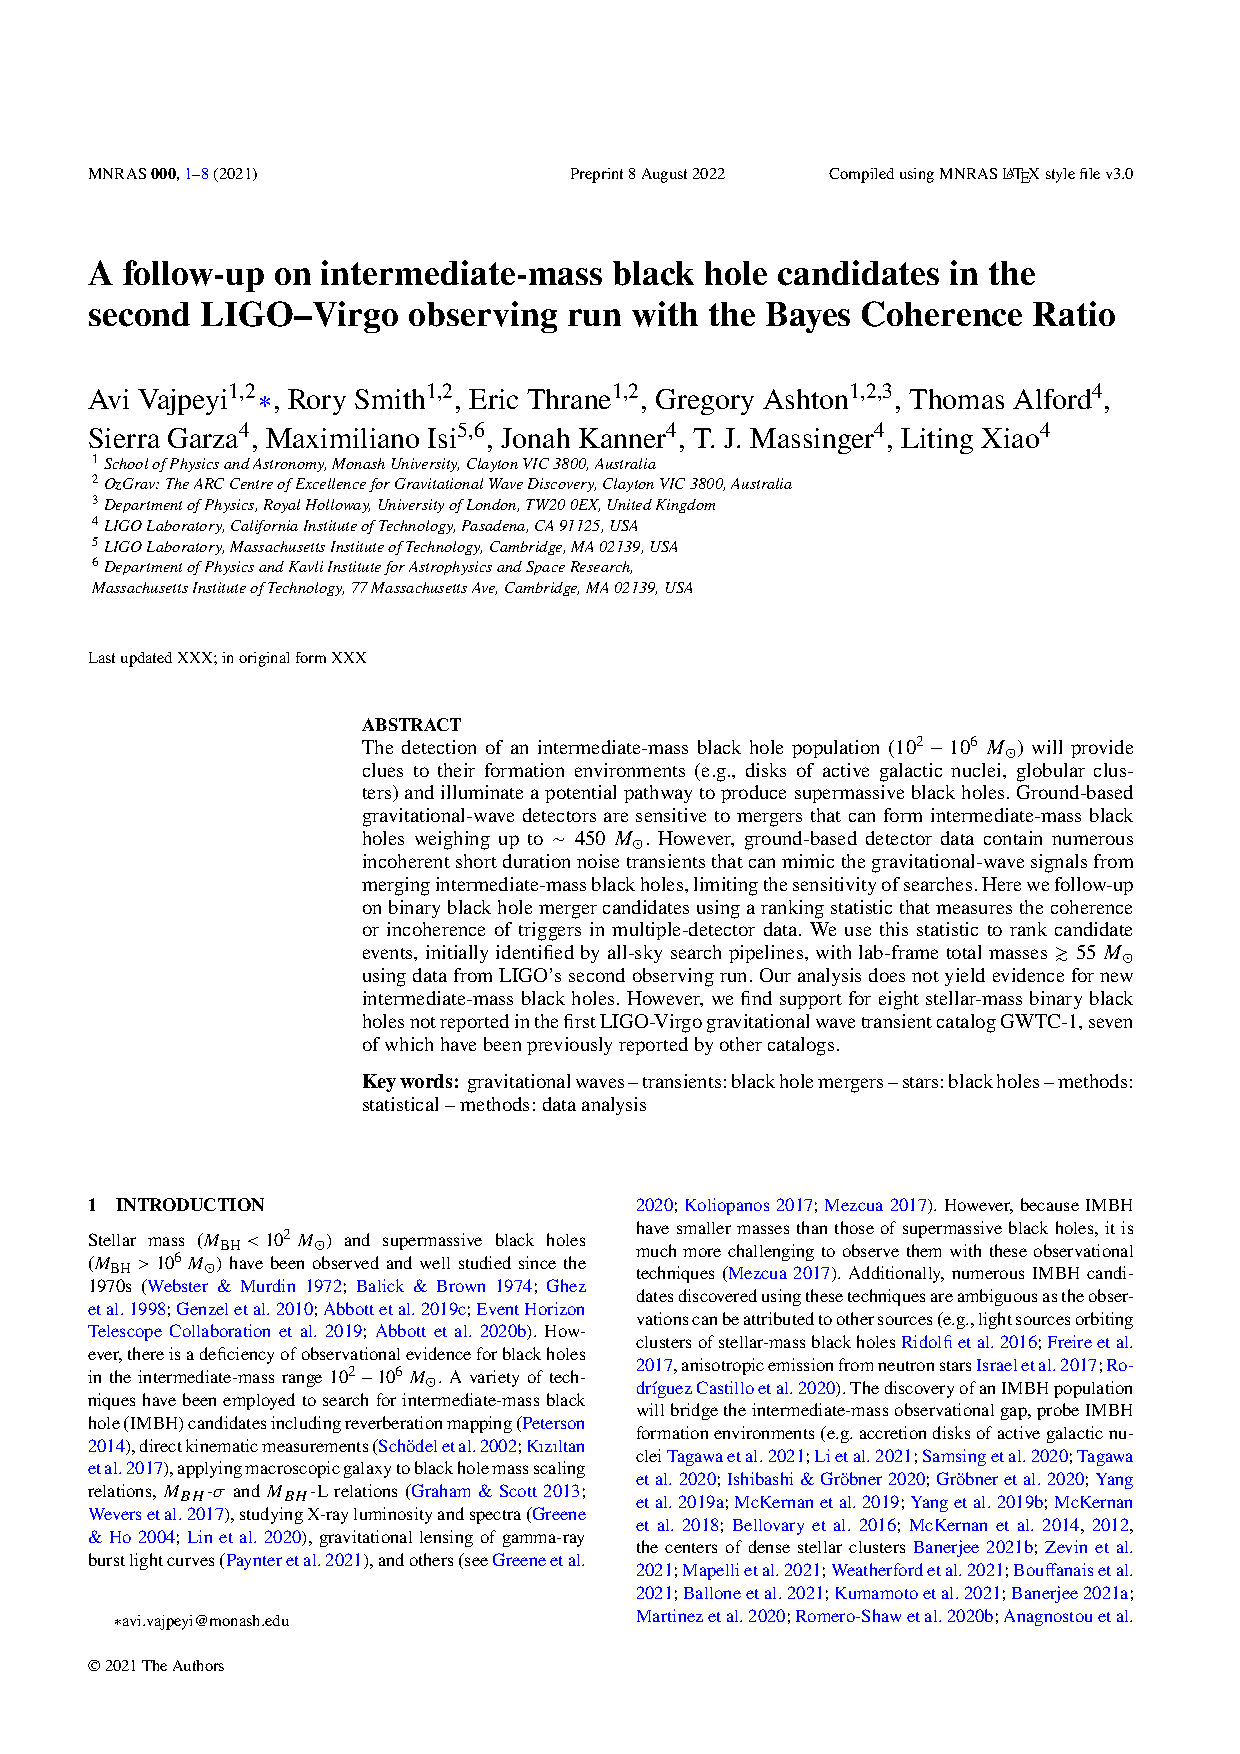
\includepdf[pages=-,pagecommand={},scale=0.93,offset=70 -40]{papers/bcr_imbh_search.pdf}

% PBilby
\chapter[Parallel Bilby]{Parallel Bilby}
\label{ch.pbilby}

\textbf{Preamble}

This chapter was originally published as:

\begin{quote}
\bibentry{pbilby}.
\end{quote}

This chapter describes \textsc{Parallel Bilby}, or \textsc{pBilby}, an opensource, parallelised implementation of \textsc{Bilby}~\cite{bilby_paper, pbilby}~\footnote{Source code available on gitlab: \url{https://git.ligo.org/lscsoft/parallel_bilby}.}. 
\textsc{pBilby} uses the Message Passing Interface \cite{mpi} to distribute samplers from \textsc{dynesty} (a nested sampling package, \cite{dynesty_paper}) over $n$-compute cores for analysis of compact-binary coalescence gravitational wave data.

Although I was not the primary author of this paper, I have played a major role in the development and maintenance of the software package \textsc{Parallal Bilby} described in this manuscript. 
Additionally, I have been leading the review of this software for the LVK. 



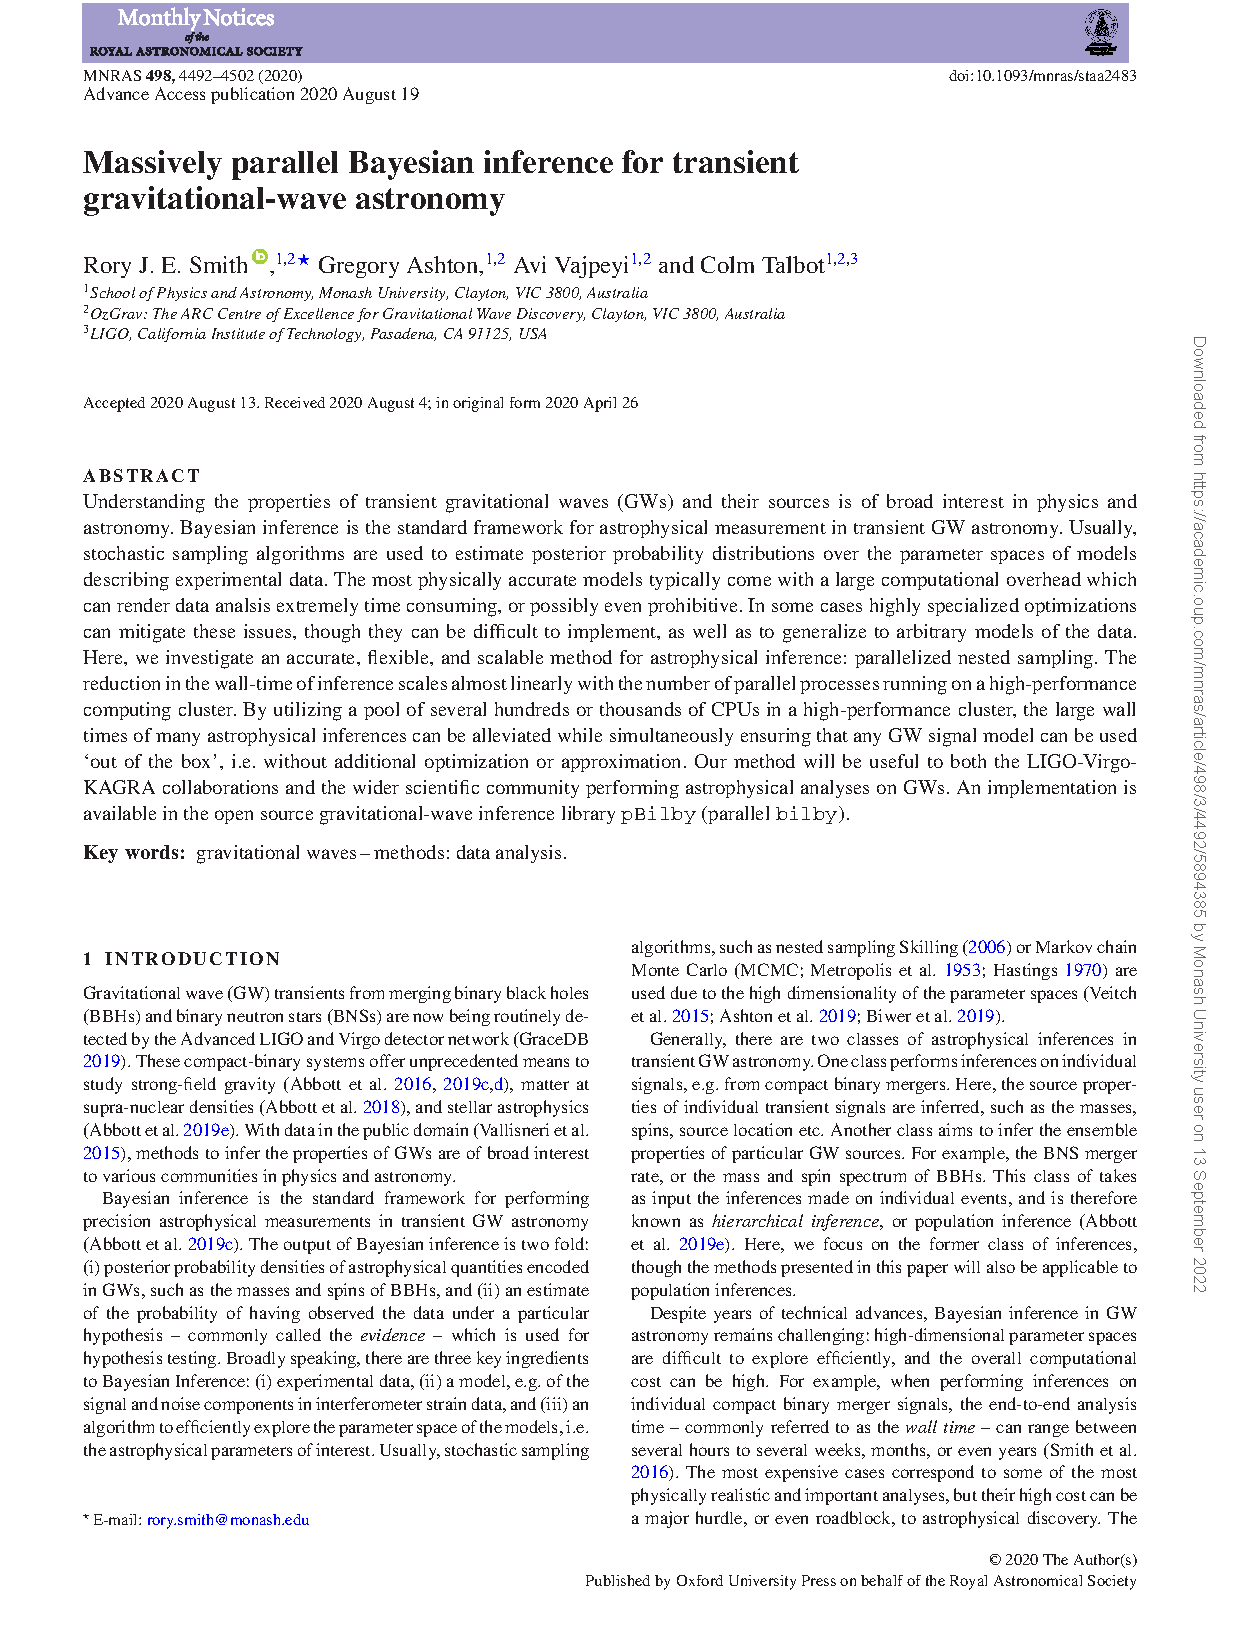
\includepdf[pages=-,pagecommand={},scale=0.93,offset=70 -80]{papers/pbilby.pdf}

% Deep Followup
\chapter[GW151226 Deep-Followup]{Deep Followup on GW151226}

This chapter was originally published as \cite{}.

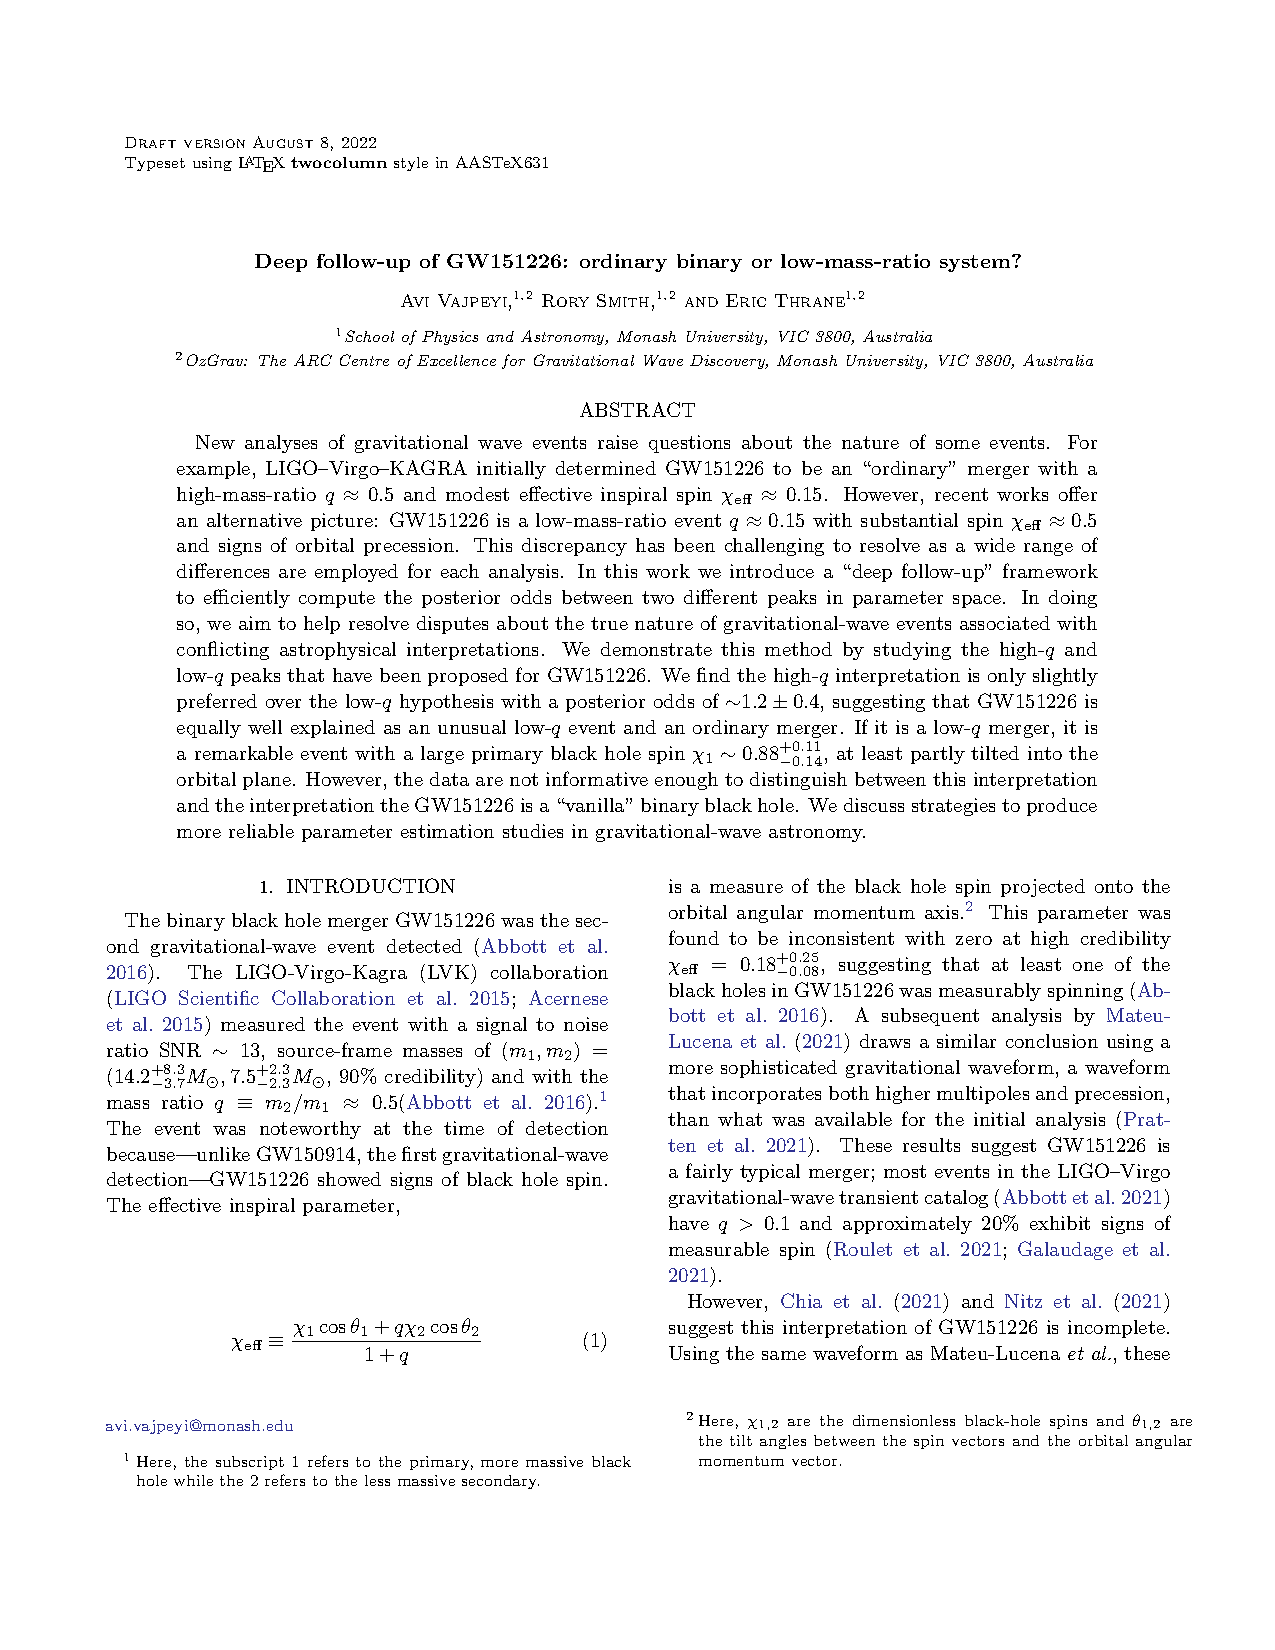
\includepdf[pages=-,pagecommand={},scale=0.93,offset=70 -40]{papers/deep.pdf}

% AGN
\chapter[BBH in AGN spin Model]{Measuring the Properties of Active Galactic Nuclei Disks with Gravitational Waves}
\label{ch.agn}

\textbf{Preamble}

This chapter was originally published as:

\begin{quote}
\bibentry{bbh_in_agn}.
\end{quote}

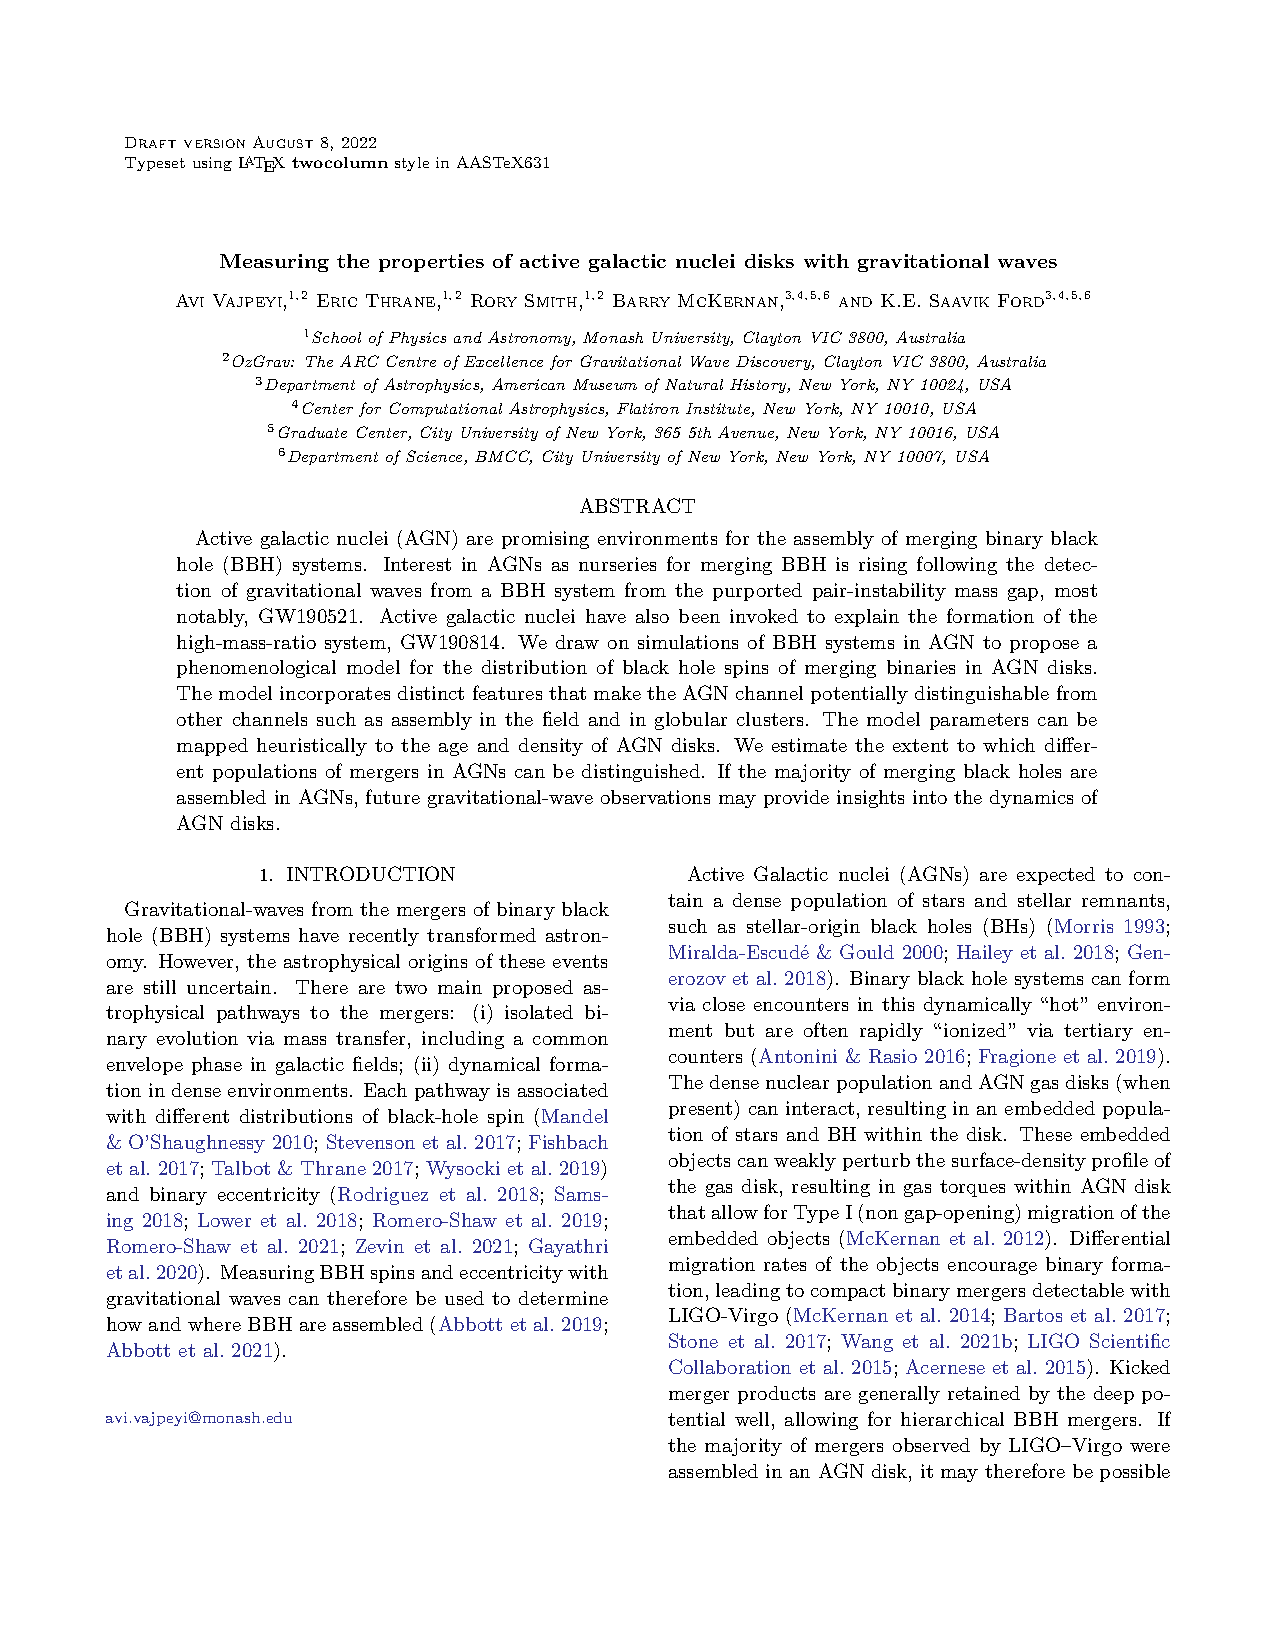
\includepdf[pages=-,pagecommand={},scale=0.93,offset=70 -45]{papers/agn.pdf}

% TESS
\chapter[TESS Atlas]{TESS Atlas}

This chapter was originally published as \cite{}.

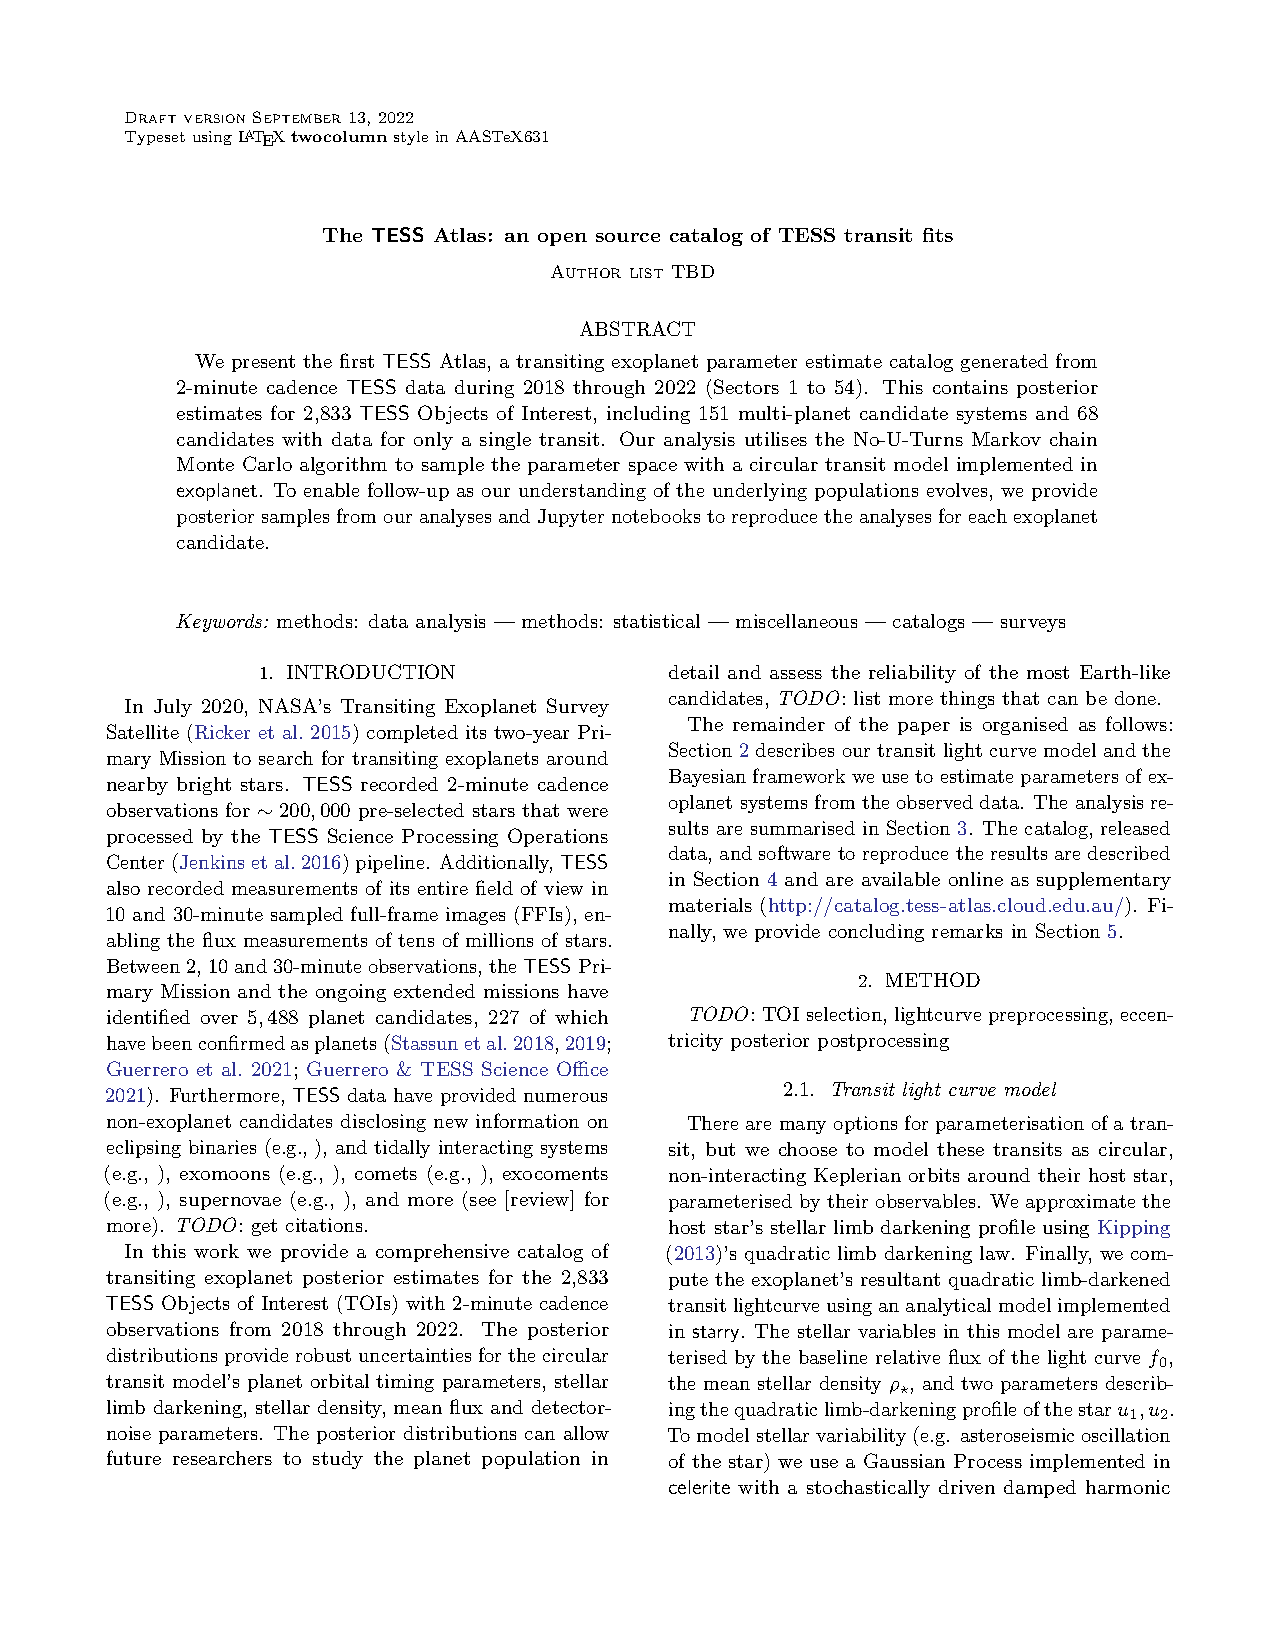
\includepdf[pages=-,pagecommand={},scale=0.93,offset=70 -40]{papers/tess_atlas.pdf}

\chapter{Summary and Conclusions}
\label{cp.conc}

Over the previous century, astronomers have moved from manual observations to automated observatories, from solitary labs to worldwide collaborations, and from catalogs containing tens of thousands of stars to those containing millions. 
It is, therefore, not surprising that scholars have begun to experiment with data-driven and computationally intensive analysis methods. This dissertation demonstrates using one of these methods, namely Bayesian inference. 
This dissertation presents the application of Bayesian inference to estimate the significance of gravitational-wave candidates with intermediate-mass black holes. 
Even though no IMBHs were discovered, the approach supports the existence of eight stellar-mass binary black holes not previously reported in the first gravitational-wave transient catalog, GWTC-1. 
In addition, the thesis proposes a novel use of Bayesian model selection for diagnosing parameter estimation outcomes. 
The diagnostic method reveals that the first GW151226 analysis was incomplete: the method finds support for an asymmetric-mass merger, previously ignored. 
The thesis also proposes a phenomenological model for AGNs that may be used to estimate AGN parameters via hierarchical Bayesian inference. 
Simulation results reveal that more than 200 events with measurable spins are necessary to use this AGN population model -- potentially achievable by the end of the next LVK observing run. 
The preceding chapter describes the first catalog of TESS candidate exoplanet parameter estimates generated via Bayesian inference. 
In the future, this catalog may assist in confirming some TESS candidates as planets. 
Finally, the dissertation describes the software to accelerate inference, which can be costly. 
This software is utilized in this thesis and by the LVK collaboration for analyzing gravitational wave events using costly models.

In the final section of this dissertation, we briefly discuss future prospects in the gravitational wave and exoplanet domains. 

\paragraph{The future of GW -- LIGO and beyond}

\begin{figure}
\begin{center}
\centerline{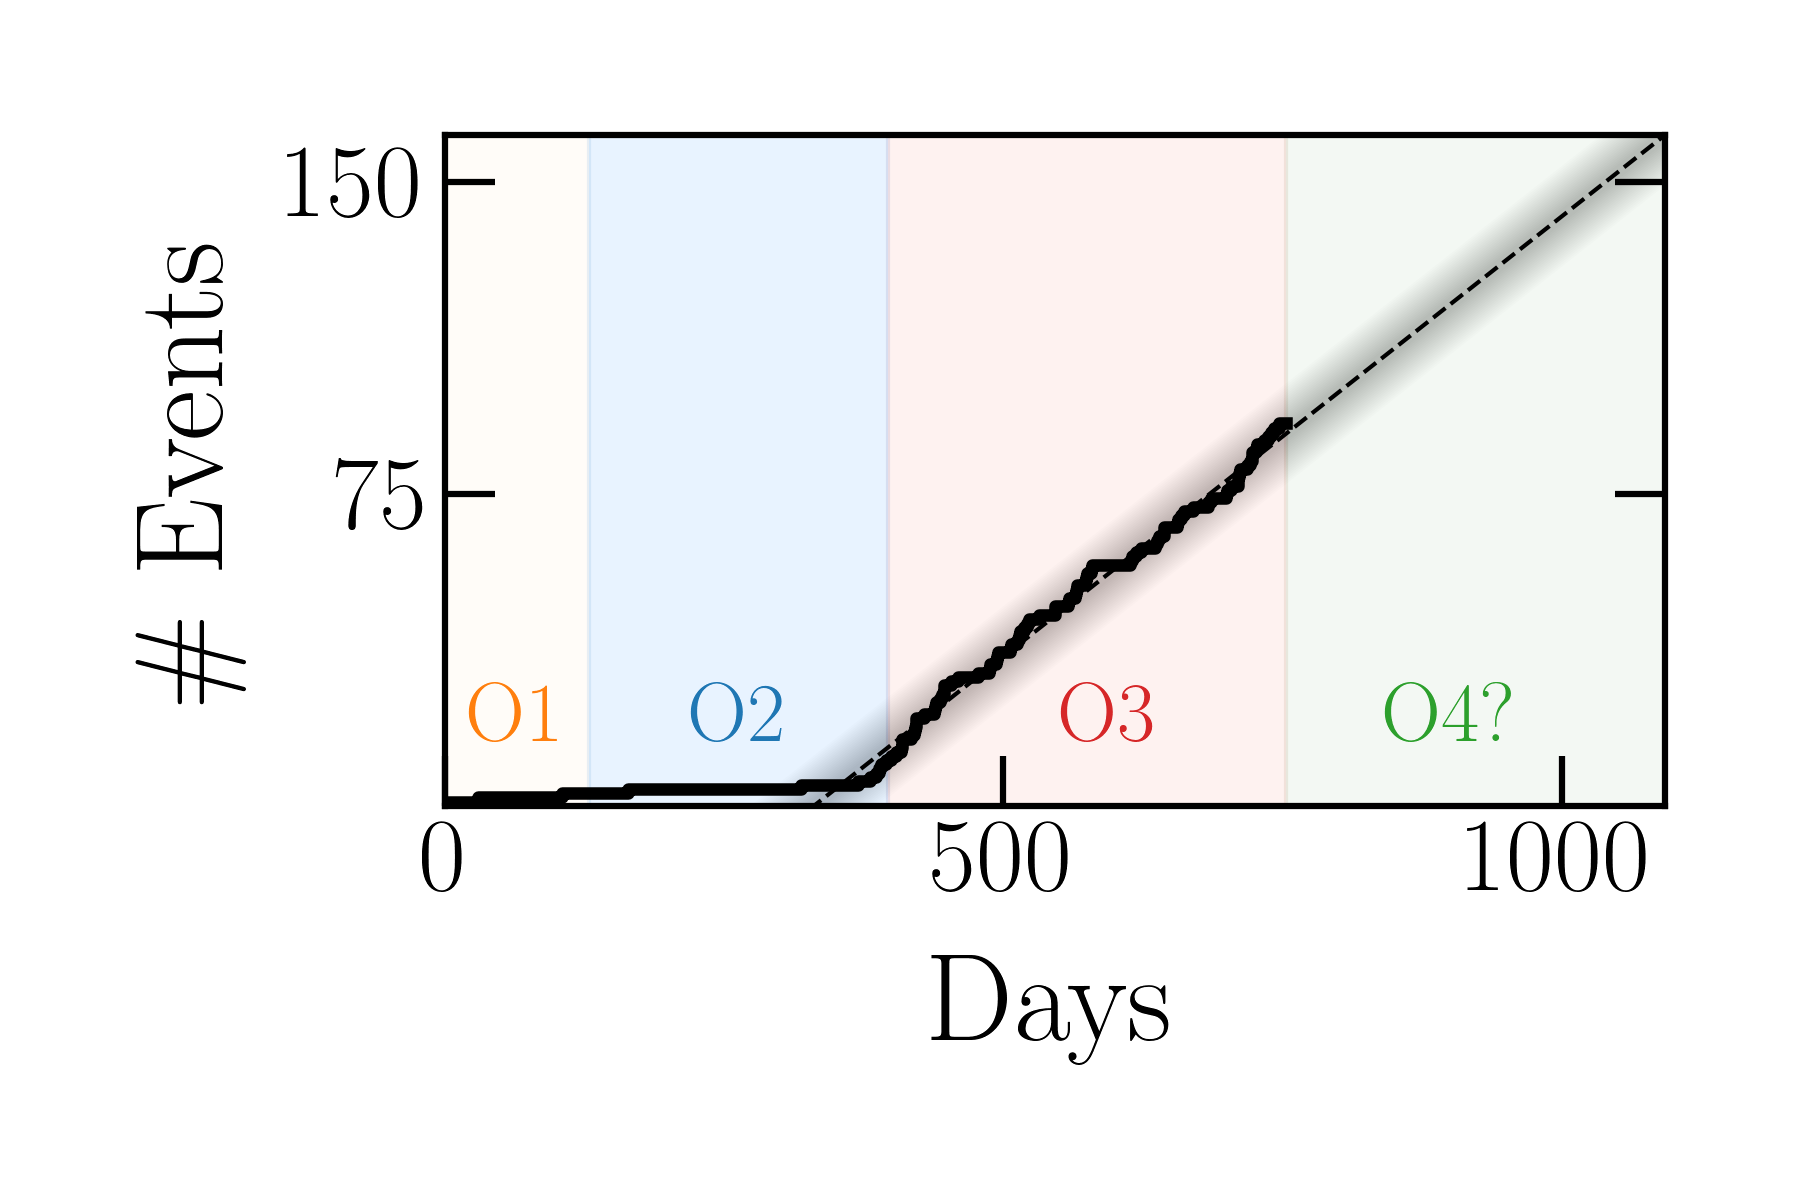
\includegraphics[width=1.\linewidth]{src/figures/gw_detection_timeframe.png}}
  \caption{\textbf{Cumulative Count of LVK Events:} The cumulative count of GW events on the vertical axis versus the number of observing days on the horizontal axis. O3 increased the count from 10 events to 93. The solid black curve is the true LVK cumulative count. The dashed black line represents an estimation of the increase in events during the fourth observing run (assuming that the O4 detection rate will be the same as O3's.  \github{https://github.com/avivajpeyi/cbc_gw_catalog_plotter}}
  \label{fig:accumulation_of_gw_events}
\end{center}
\end{figure}

The LIGO, VIRGO and KAGRA detectors have made GW astronomy a reality. 
Over the past eight years, the detections made have been a scientific goldmine. 
The detections have allowed us to study black hole mass spectrum~\cite{}, test general relativity~\cite{}, measure cosmological parameters~\cite{} and probe various neutron-star equation of state~\cite{}. 
Soon, the next LVK observing run, O4, will provide astronomers with more events two study the universe with. 
Figure~\ref{fig:accumulation_of_gw_events} shows the increase in GW events over the first three observing runs. 
It also provides a conservative estimate of the number of events in O4 (more detections are expected due to the detector upgrades).
However, even with the events that might be detected by the end of O4 and O5, the current GW detectors can only provide a glimpse of the full gravitational-wave universe. 

The next generation  of detectors will broaden this view. 
Plans of ground based detectors such as CE (Cosmic Explorer) and ET (Einstein Telescope), and even the spaced based detector LISA(Laser Interferometer Space Antenna) have been progressing in a positive direction. 
LISA will permit gravitational wave astronomers to study an entirely new spectrum of gravitational waves. 
For example, LISA will allow us to probe the merger of massive and supermassive black holes, and inspirals of compact objects such as white dwarf stars and neutron stars. 
The next generation ground based detectors (XG) will probe the same gravitational wave spectrum as the current LVK detectors. 
However, the XG detectrs will be over ten times more sensitive than the current detectors~\cite{}. 
Figure~\ref{fig:ligo_vs_ce} compares the sensitivity of CE and LIGO A+ (advanced LIGO). 
As shown in Figure~\ref{fig:ligo_vs_ce}a while the maximum distance the LIGO A+ can probe is $z\sim10$, CE can probe gravitational-wave astronomy from the edge of the observable universe $z\sim100$. 
This will allow astronomers to study the black hole mass spectrum as a function of redshift, and possible find primordial black holes.
\begin{figure}
\begin{center}
  \centerline{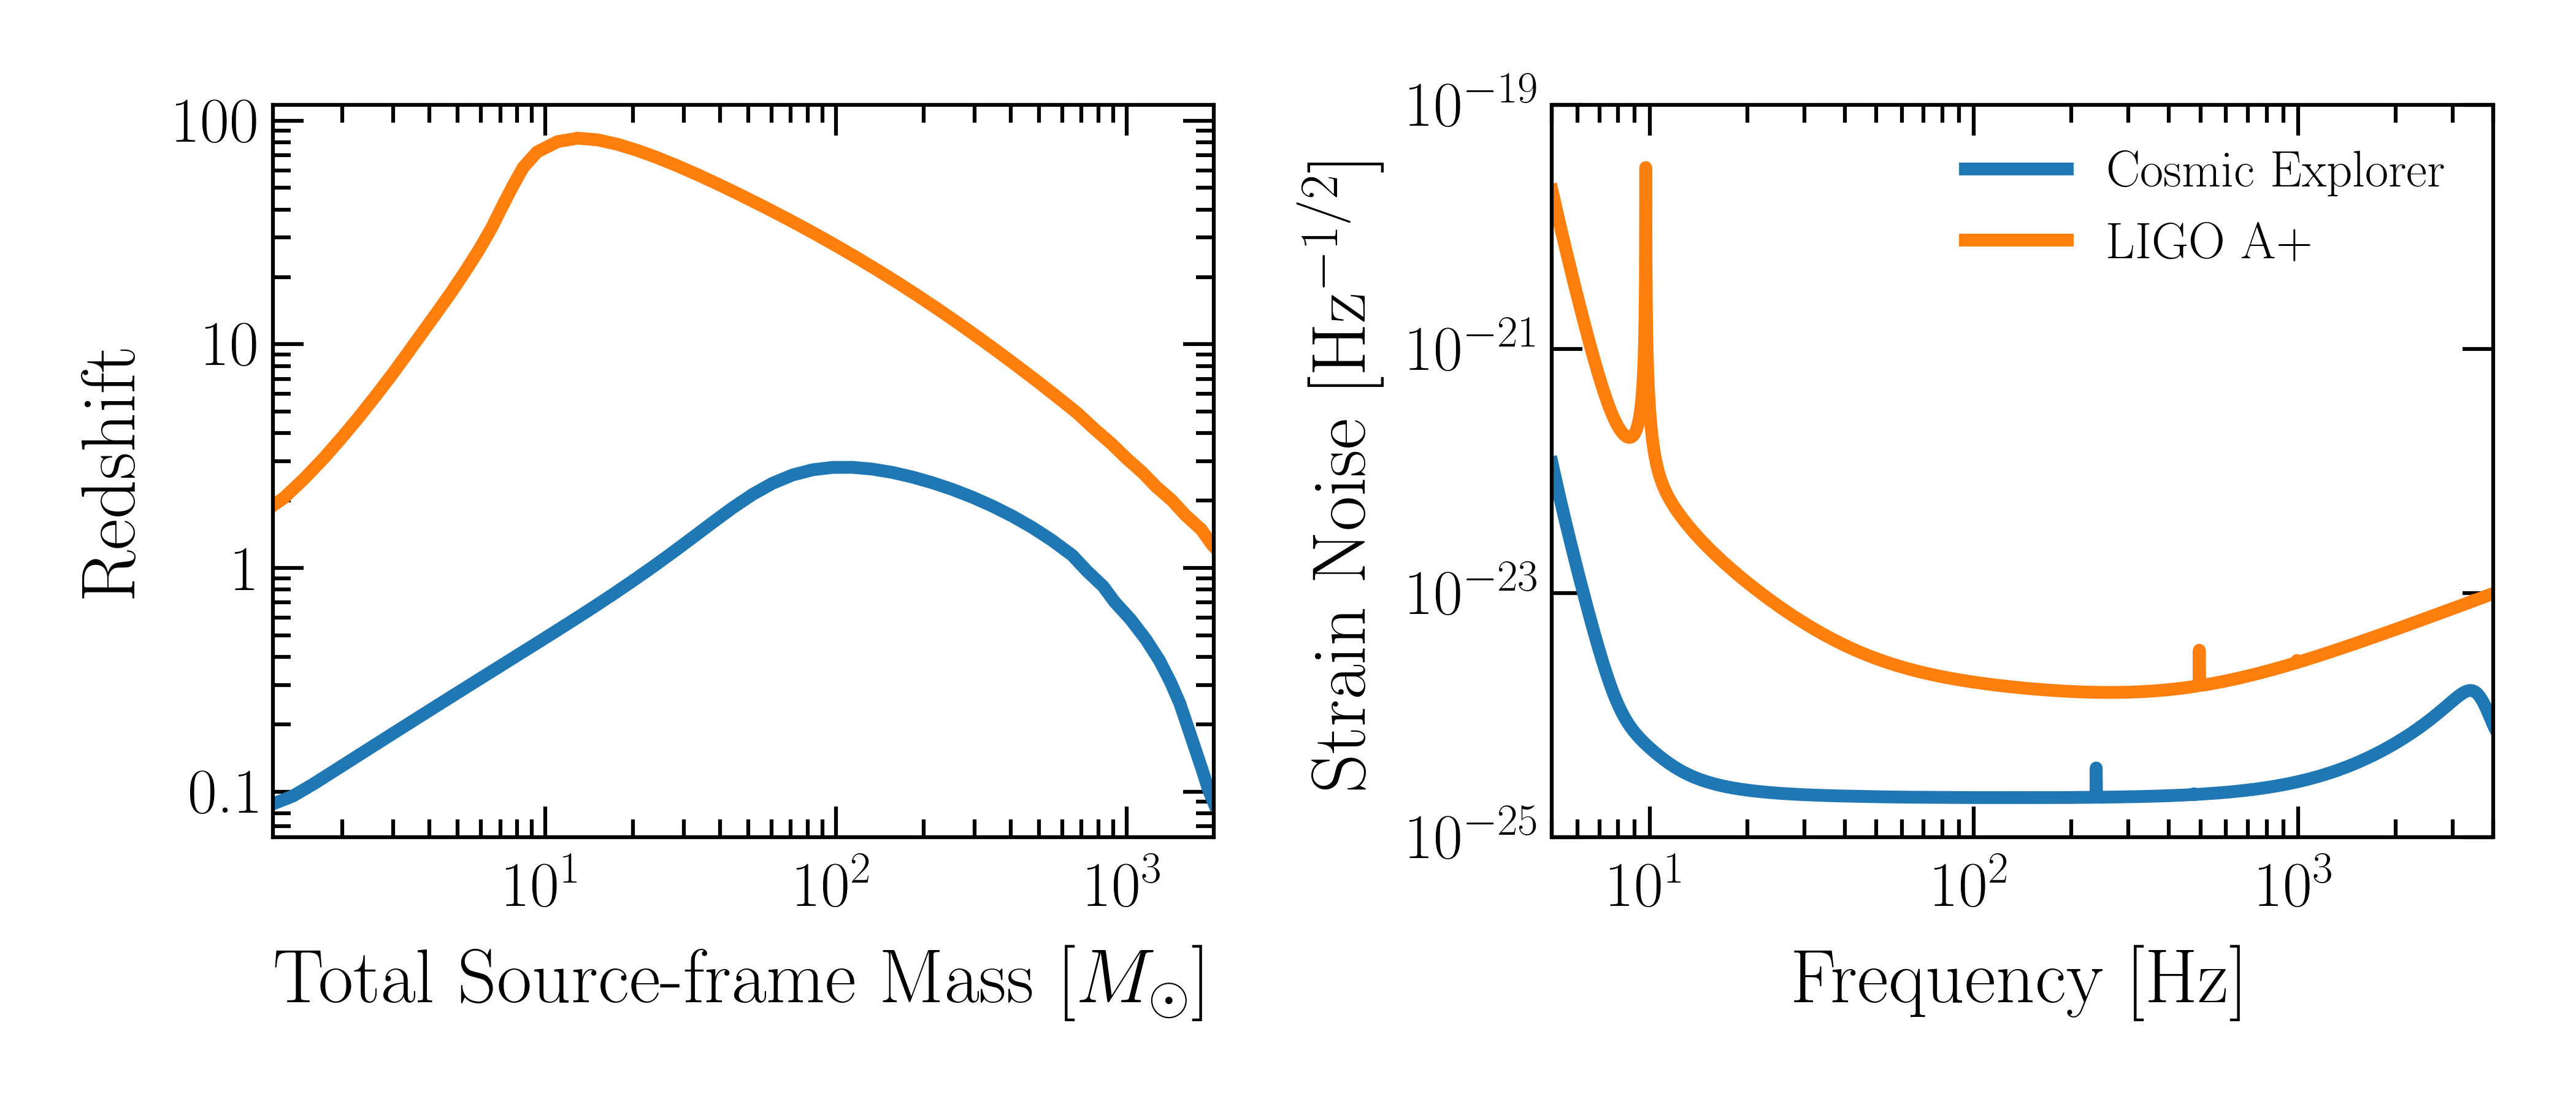
\includegraphics[width=1.\linewidth]{src/figures/ligo_vs_ce.png}}
  \caption{\textbf{LIGO A+ and CE Comparisons:}  \github{https://github.com/avivajpeyi/cbc_gw_catalog_plotter}}
  \label{fig:ligo_vs_ce}
\end{center}
\end{figure}


\paragraph{Probing habitable exoplanet atmospheres}
The next frontier for inquiry is characterizing the atmospheres of exoplanets. 
It's the next step toward finding life. 
Exoplanets have a similar driver larger than pure scientific curiosity. 
The ultimate goal
for many researchers is the search for habitable exoplanets. 
The exoplanet atmosphere
is the only way to infer whether or not a planet is habitable or likely inhabited; the
planetary atmosphere is our window into temperatures, habitability indicators, and
biosignature gases.


% https://www.annualreviews.org/doi/full/10.1146/annurev-astro-112420-020055

The Nancy Grace Roman Space Telescope, expected to launch in 2027, will make new exoplanet discoveries using a variety of methods. The ESA (European Space Agency) mission ARIEL, launching in 2029, will observe exoplanet atmospheres; a piece of NASA technology aboard, called CASE, will help zero in on exoplanet clouds and hazes

% The James Webb Space Telescope, which was not built to study exoplanets but to look for the oldest stars in the universe, has already delivered a string of breakthroughs in exoplanet research, including detecting carbon dioxide and water in the atmospheres of several of them. Quanz, however, cautions that Webb, although the most powerful observatory ever put to space, is not quite powerful enough to be able to see the much smaller, Earth-like planets that orbit closer to their stars at distances where liquid water can exist.



% Now that we have found exoplanets, the next frontier for inquiry is characterizing the atmospheres of exoplanets.
% +
% +Characterizing the atmospheres of exoplanets is the next frontier for inquiry because it allows us to learn more about the conditions on those planets. By studying the atmospheric composition, we can learn about the planet's climate and potential habitability. Additionally, studying the atmospheres of exoplanets can help us to better understand how planets form and evolve.

% The goal is to use TESS data to hopefully identify a possible "Goldilocks" situation: an exoplanet similar to Earth, in an orbit at which position liquid water could exist on the surface, and thus which could have the basics for life to develop. We're still a long way from being able to visit such exoplanets, but TESS' data has already helped develop a shortlist of potential candidates.

% Read More: https://www.slashgear.com/after-two-astonishing-years-nasas-tess-is-onto-the-next-exoplanet-hunt-11633044/?utm_campaign=clip


Wolszczan, who still searches for exoplanets as a professor at Penn State, says we’re opening an era of discovery that will go beyond simply adding new planets to the list. The Transiting Exoplanet Survey Satellite (TESS), launched in 2018, continues to make new exoplanet discoveries. But soon powerful next-generation telescopes and their highly sensitive instruments, starting with the recently launched James Webb Space Telescope, will capture light from the atmospheres of exoplanets, reading which gases are present to potentially identify tell-tale signs of habitable conditions.

The Nancy Grace Roman Space Telescope, expected to launch in 2027, will make new exoplanet discoveries using a variety of methods. The ESA (European Space Agency) mission ARIEL, launching in 2029, will observe exoplanet atmospheres; a piece of NASA technology aboard, called CASE, will help zero in on exoplanet clouds and hazes.


% https://www.nasa.gov/feature/jpl/cosmic-milestone-nasa-confirms-5000-exoplanets

%% ----------------------------------------------------------------
% Now begin the Appendices, including them as separate files

\addtocontents{toc}{\vspace{2em}} % Add a gap in the Contents, for aesthetics

% \appendix % Cue to tell LaTeX that the following 'chapters' are Appendices
%
% \input{Appendices/AppendixA}	% Appendix Title


\addtocontents{toc}{\vspace{2em}}  % Add a gap in the Contents, for aesthetics
\backmatter

%% ----------------------------------------------------------------
\label{Bibliography}
\lhead{\emph{Bibliography}}  % Change the left side page header to "Bibliography"
\bibliographystyle{unsrtnat}  % Use the "unsrtnat" BibTeX style for formatting the Bibliography
\bibliography{bibliography}  % The references (bibliography) information are stored in the file named "Bibliography.bib"

\end{document}  % The End
%% ----------------------------------------------------------------
